% !TeX program = lualatex
% Für echtes Arial/Calibri: lualatex/xelatex + biber verwenden.
% Fallback mit pdflatex funktioniert (sans: TeX Gyre Heros).

\documentclass[11pt,a4paper]{article}

% ---------- Pakete: Sprache, Schrift, Mikrotypografie ----------
\usepackage[a4paper,margin=2cm]{geometry} % 2,00 cm Ränder
\usepackage[ngerman,english]{babel}       % Silbentrennung DE/EN
\usepackage{microtype}                    % Mikrotypografie (Silbentrennung/Zeilenumbrüche)
\usepackage[T1]{fontenc}
\usepackage[utf8]{inputenc}
\usepackage{iftex}
\ifPDFTeX
% Fallback: pdfLaTeX (Arial-ähnlich)
\usepackage[scale=0.95]{tgheros}   % TeX Gyre Heros ~ Helvetica/Arial
\renewcommand{\familydefault}{\sfdefault}
\else
% Echte Systemschriften mit Lua/XeLaTeX:
\usepackage{fontspec}
\usepackage{xcolor}
\setmainfont{Arial}[
Ligatures=TeX,
Scale=1.0
]
% Optionaler alternativer Sans-Font:
% \setmainfont{Calibri}[Ligatures=TeX,Scale=1.0]
\fi

% ---------- Zeilen & Absätze ----------
\usepackage{setspace}
\onehalfspacing                           % 1,5-zeilig
\setlength{\parindent}{0pt}               % kein Einzug
\setlength{\parskip}{6pt}                 % 6 pt Abstand nach Absatz

% ---------- Mathe, Grafik, Tabellen ----------
\usepackage{amsmath,amssymb}
\usepackage{graphicx}
\usepackage{booktabs}
\usepackage{float}
\usepackage{subcaption}
\usepackage{siunitx}
\sisetup{detect-all}                      % Sans-Serif in siunitx
\usepackage{csquotes}                     % saubere Anführungszeichen / Blockzitate
\usepackage{mwe}                          % Beispielbilder (example-image*)

% ---------- Code ----------
\usepackage{listings}

% dezente Farben
\definecolor{lwbg}{rgb}{0.98,0.98,0.98}     % leichter Hintergrund
\definecolor{lwkeyword}{rgb}{0.0,0.45,0.30} % keywords (dezent grün)
\definecolor{lwcomment}{rgb}{0.45,0.45,0.45}
\definecolor{lwstring}{rgb}{0.5,0.15,0.15}

\lstdefinestyle{python-academic}{
    language=Python,
    backgroundcolor=\color{lwbg},
    basicstyle=\ttfamily\small,        % gut lesbare Größe im Fließtext
    numbers=left,
    numberstyle=\tiny\color{gray},
    stepnumber=1,
    numbersep=8pt,
    frame=single,                      % klarer, aber dezenter Rahmen
    rulecolor=\color{black!20},
    tabsize=4,
    breaklines=true,
    breakatwhitespace=false,
    showstringspaces=false,
    captionpos=b,
    aboveskip=6pt,
    belowskip=6pt,
    xleftmargin=4pt,
    keywordstyle=\bfseries\color{lwkeyword},
    commentstyle=\itshape\color{lwcomment},
    stringstyle=\color{lwstring},
    upquote=true,                      % gerade quotes, falls nötig
    escapeinside={(*@}{@*)},           % für LaTeX-Math etc. im Listing
}

\lstset{style=python-academic}

% Nutzung: entweder inline
% \begin{lstlisting}[caption={Minimalbeispiel},label={lst:mini}]
    % def foo(x):
    %     return x**2
    % \end{lstlisting}
%
% oder aus Datei:
% \lstinputlisting[language=Python, caption={Script X}, label={lst:scriptx}]{path/to/script.py}

% ---------- Bild-/Tabellenunterschriften (10 pt) ----------
\usepackage{caption}
\captionsetup{font=footnotesize,labelfont=bf,labelsep=colon}
\addto\captionsngerman{\renewcommand{\figurename}{Abb.}}
\addto\captionsngerman{\renewcommand{\tablename}{Tab.}}
\newcommand{\source}[1]{\caption*{\footnotesize #1}} % Quellenangabe 10 pt

% ---------- Überschriften: Größen/Abstände/Nummerntiefe ----------
\usepackage{titlesec}
% H1: 16 pt, 12/12
\titleformat{\section}{\bfseries\fontsize{16pt}{18pt}\selectfont}{\thesection}{0.6em}{}
\titlespacing*{\section}{0pt}{12pt}{12pt}
% H2: 14 pt, 12/6
\titleformat{\subsection}{\bfseries\fontsize{14pt}{16pt}\selectfont}{\thesubsection}{0.6em}{}
\titlespacing*{\subsection}{0pt}{12pt}{6pt}
% H3: 11 pt, 12/6
\titleformat{\subsubsection}{\bfseries\fontsize{11pt}{13pt}\selectfont}{\thesubsubsection}{0.6em}{}
\titlespacing*{\subsubsection}{0pt}{12pt}{6pt}
\setcounter{secnumdepth}{3}
\setcounter{tocdepth}{3}

% Jede Section (Ebene 1) startet auf neuer Seite
\usepackage{etoolbox}
\pretocmd{\section}{\clearpage}{}{}

% ---------- Inhaltsverzeichnis: nur Ebene 1 fett ----------
\usepackage{tocloft}
\renewcommand{\cftsecfont}{\bfseries}
\renewcommand{\cftsecpagefont}{}

% ---------- Fußnoten explizit 10 pt ----------
\makeatletter
\renewcommand\footnotesize{\@setfontsize\footnotesize{10pt}{12pt}}
\makeatother

% ---------- Seitenzahlen: zentriert im Fuß ----------
\usepackage{fancyhdr}
\pagestyle{fancy}
\fancyhf{}
\cfoot{\thepage}

% ---------- Hyperlinks schwarz (keine Farben/Rahmen) ----------
\usepackage[hidelinks]{hyperref}

% ---------- APA7 Literatur (Biber) + deutscher Mapping ----------
\usepackage[
style=apa,
backend=biber,
sorting=nyt,
uniquename=init,
maxcitenames=2, % "et al." ab 3
maxbibnames=99,
doi=true,
url=true,
dateabbrev=false, % Vollständige Datumsangaben
eprint=false, % Unterdrücke eprint-Felder wenn DOI vorhanden
isbn=false, % ISBN normalerweise nicht in APA7
giveninits=true % Nur Initialen für Vornamen
]{biblatex}
\DeclareLanguageMapping{ngerman}{ngerman-apa}

% Zusätzliche APA7-Konfigurationen
\ExecuteBibliographyOptions{maxbibnames=999} % Alle Autoren im Literaturverzeichnis
\ExecuteBibliographyOptions{giveninits=true} % Nur Initialen
\ExecuteBibliographyOptions{uniquename=init} % Eindeutigkeit durch Initialen

% DOI-Formatierung anpassen
\DeclareFieldFormat{doi}{%
  \mkbibacro{DOI}\addcolon\space
  \ifhyperref
    {\href{https://doi.org/#1}{\nolinkurl{#1}}}
    {\nolinkurl{#1}}}

% Hängender Einzug 1.27 cm, 1,5-zeilig wie Text
\setlength{\bibhang}{1.27cm}
\defbibenvironment{bibliography}
{\list
    {\printtext[labelnumberwidth]{\printfield[labelnumberwidth]{labelnumber}}}
    {\setlength{\leftmargin}{\bibhang}
        \setlength{\itemindent}{-\bibhang}
        \setlength{\itemsep}{\baselineskip} % 1.5-Zeilenabstand wie Text
        \setlength{\parsep}{0pt}}
    \renewcommand*{\makelabel}[1]{##1\hss}}
{\endlist}
{\item}

% Beispiel-Bibliothek im Dokument (kannst du ersetzen)
\begin{filecontents*}{\jobname.bib}
    @book{Goodfellow2016,
        author    = {Goodfellow, Ian and Bengio, Yoshua and Courville, Aaron},
        year      = {2016},
        title     = {Deep Learning},
        publisher = {MIT Press},
        address   = {Cambridge, MA},
        isbn      = {978-0262035613}
    }
    @book{Bishop2006,
        author    = {Bishop, Christopher M.},
        year      = {2006},
        title     = {Pattern Recognition and Machine Learning},
        publisher = {Springer},
        address   = {New York, NY},
        doi       = {10.1007/978-0-387-45528-0}
    }
    @book{Hastie2009,
        author    = {Hastie, Trevor and Tibshirani, Robert and Friedman, Jerome},
        year      = {2009},
        title     = {The Elements of Statistical Learning},
        subtitle  = {Data Mining, Inference, and Prediction},
        edition   = {2},
        publisher = {Springer},
        address   = {New York, NY},
        doi       = {10.1007/978-0-387-84858-7}
    }
    @article{Kingma2015,
        author  = {Kingma, Diederik P. and Ba, Jimmy},
        year    = {2015},
        title   = {Adam: A Method for Stochastic Optimization},
        journaltitle = {Proceedings of the 3rd International Conference on Learning Representations},
        venue   = {San Diego, CA},
        eprint  = {1412.6980},
        eprinttype = {arxiv},
        url     = {https://arxiv.org/abs/1412.6980}
    }
    @incollection{Platt1999,
        author    = {Platt, John},
        year      = {1999},
        title     = {Probabilistic Outputs for Support Vector Machines and Comparisons to Regularized Likelihood Methods},
        booktitle = {Advances in Large Margin Classifiers},
        editor    = {Smola, Alexander J. and Bartlett, Peter and Schölkopf, Bernhard and Schuurmans, Dale},
        publisher = {MIT Press},
        address   = {Cambridge, MA},
        pages     = {61--74}
    }
    @online{Mueller2023,
        author = {Müller, Andreas and Schmidt, Maria},
        year   = {2023},
        title  = {Aktuelle Entwicklungen im Machine Learning},
        url    = {https://example.com/ml-trends},
        urldate = {2024-01-15}
    }
\end{filecontents*}
\addbibresource{Praxisprojekt_4.bib}

% ---------- Automatische Verzeichnisse nur bei ≥3 Einträgen ----------
\usepackage{totcount}
\regtotcounter{figure}
\regtotcounter{table}
\newcommand{\addtoTOC}[1]{\addcontentsline{toc}{section}{#1}}
\newcommand{\printlistsconditional}{%
    % Wirksam nach erneutem LaTeX-Lauf (Zähler aus .aux):
    \ifnum\totvalue{figure}>2
    \renewcommand{\listfigurename}{Abbildungsverzeichnis}
    \listoffigures
    \addtoTOC{Abbildungsverzeichnis}
    \clearpage
    \fi
    \ifnum\totvalue{table}>2
    \renewcommand{\listtablename}{Tabellenverzeichnis}
    \listoftables
    \addtoTOC{Tabellenverzeichnis}
    \clearpage
    \fi
}

% ---------- Blockzitat ≥ 40 Wörter (APA) ----------
\newenvironment{blockzitat}{%
    \begin{quote}\setlength{\leftskip}{1.27cm}\itshape\upshape\mdseries\selectfont
    }{\end{quote}}

% ---------- Meta-Felder für Titelseite ----------
\newcommand{\university}{Internationale Hochschule Duales Studium}
\newcommand{\studyprogram}{B.Sc. Informatik}
\newcommand{\thesistype}{Projektarbeit}
\newcommand{\papertitle}{Inwieweit sind Machine-Learning-Modelle für Netzwerk-Anomalieerkennung zwischen verschiedenen Datensätzen übertragbar?}
\newcommand{\authorname}{Jonas Weirauch}
\newcommand{\matno}{10237021}
\newcommand{\address}{Im Wiesengrund 19, 55286 Sulzheim}
\newcommand{\advisor}{Dominic Lindner}
\newcommand{\submissiondate}{30.09.2025}

% ============================================================
%                         DOKUMENT
% ============================================================
\begin{document}
    \selectlanguage{ngerman}

    % ---------- Titelblatt (zählt als I, ohne Zahl) ----------
    \pagenumbering{Roman}
    \setcounter{page}{1}
    \begin{titlepage}
        \thispagestyle{empty}
        \vspace*{-1cm}
        
        % IU Logo
        \begin{center}
            \includegraphics[width=5cm]{/home/jonas/Documents/Studium/Allgemein/IU_Logo.png}
        \end{center}
        
        \vspace{3cm}
        
        % Projektarbeit
        \begin{center}
            {\fontsize{11pt}{13pt}\selectfont \thesistype}
        \end{center}
        
        \vspace{2cm}
        
        % University and Program
        \begin{center}
            {\fontsize{11pt}{13pt}\selectfont \university}
            
            \vspace{0.5cm}
            
            {\fontsize{11pt}{13pt}\selectfont Studiengang: \studyprogram}
        \end{center}
        
        \vspace{2cm}
        
        % Title
        \begin{center}
            {\bfseries\fontsize{12pt}{14pt}\selectfont \papertitle}
        \end{center}
        
        \vspace{2cm}
        
        % Author details
        \begin{center}
            {\fontsize{11pt}{13pt}\selectfont \authorname}
            
            {\fontsize{11pt}{13pt}\selectfont Matrikelnummer: \matno}
            
            {\fontsize{11pt}{13pt}\selectfont \address}
        \end{center}
        
        \vspace{2cm}
        
        % Supervisor and date
        \begin{center}
            {\fontsize{11pt}{13pt}\selectfont Betreuende Person: \advisor}
            
            {\fontsize{11pt}{13pt}\selectfont Abgabedatum: \submissiondate}
        \end{center}
        
        \vfill
    \end{titlepage}

    % ---------- Erklärung / Sperrvermerk (optional je nach Arbeit) ----------
%    \section*{Erklärung / Sperrvermerk}
%    \addtoTOC{Erklärung / Sperrvermerk}
%    Hier ggf. die Eigenständigkeits- und Sperrvermerkserklärung gemäß Vorgaben der Hochschule.
%    \clearpage

    % ---------- Danksagung (optional) ----------
%    \section*{Danksagung}
%    \addtoTOC{Danksagung}
%    Optionaler Text für Danksagungen.
%    \clearpage

    % ---------- Abstracts (Deutsch & Englisch, je ca. 200 Wörter) ----------
%    \section*{Abstract (Deutsch)}
%    \addtoTOC{Abstract (Deutsch)}
%    Kurzfassung der Arbeit (ca. 200 Wörter): Problemstellung, Methode, Ergebnisse, Implikationen.
%    \clearpage

%    \begin{otherlanguage*}{english}
%        \section*{Abstract (English)}
%        \addtoTOC{Abstract (English)}
%        Abstract (approx. 200 words): problem, method, results, implications.
%    \end{otherlanguage*}
%    \clearpage

    % ---------- Inhaltsverzeichnis ----------
    \renewcommand{\contentsname}{Inhaltsverzeichnis}
    \tableofcontents
    \clearpage

    % ---------- Abbildungs-/Tabellenverzeichnis (nur bei ≥3) ----------
    \printlistsconditional

    % ---------- Abkürzungsverzeichnis ----------
    \section*{Abkürzungsverzeichnis}
    \addtoTOC{Abkürzungsverzeichnis}
    \begin{tabular}{@{}ll}
        \textbf{AI}  & Artificial Intelligence \\
        \textbf{DoS} & Denial-of-Service \\
        \textbf{IDS} & Intrusion Detection Systems \\
        \textbf{ML}  & Machine Learning \\
    \end{tabular}
    \clearpage

    % ---------- Hauptteil: arabische Seitenzahlen ab "Einleitung" ----------
    \pagenumbering{arabic}
    \setcounter{page}{1}

    \section{Einleitung}
    \subsection{Motivation und Problemstellung}

    Mit über 10,5 Billionen US-Dollar geschätzten jährlichen Schäden bis 2025 stellen Cyberangriffe eine der größten globalen Bedrohungen dar \parencite{GlobalRisksReport2024}. Gemäß dem Global Risk Report 2024 des Weltwirtschaftsforums gehören Cyberangriffe zu den fünf bedeutendsten globalen Risiken in den nächsten Jahren, was einer Verdreifachung der finanziellen Verluste im Vergleich zu 2015 entspricht \parencite{GlobalRisksReport2024}. Diese besorgniserregenden Statistiken unterstreichen die akute Notwendigkeit wirksamer Sicherheitsvorkehrungen zum Schutz kritischer Infrastrukturen \parencite{Taman2024}.

    Traditionelle signaturbasierte Intrusion Detection Systeme (IDS) erreichen zunehmend ihre Grenzen bei der Erkennung neuartiger Zero-Day-Exploits und unbekannter Angriffsmuster \parencite{Ring2019,Belavagi2016}. Diese Systeme können lediglich bekannte Signaturen identifizieren und versagen bei der Detektion innovativer Bedrohungen. Gleichzeitig führen die steigende Vernetzung und Digitalisierung zu einer kontinuierlichen Zunahme der Angriffsvektoren und einer erhöhten Komplexität der Netzwerkumgebungen.

    Machine Learning (ML) bietet das Potenzial, diese Limitationen zu überwinden und auch bisher unbekannte Angriffsmuster aufzudecken \parencite{Vinayakumar2019}. Dennoch ist die tatsächliche Wirksamkeit verschiedener ML-Modelle in heterogenen Netzwerken noch nicht vollständig geklärt. Ein kritisches Problem stellt dabei die Generalisierungsfähigkeit dar: Während Modelle auf spezifischen Trainingsdaten exzellente Leistungen erzielen, zeigen sie oft dramatische Leistungseinbußen beim Transfer auf neue Netzwerkumgebungen oder unterschiedliche Datensätze \parencite{Ring2019}.

    \subsection{Forschungsfrage und Zielsetzung}

    Diese Arbeit untersucht systematisch die Generalisierungsfähigkeit von zwölf ML-Modellen über zwei fundamental unterschiedliche Netzwerk-Datensätze hinweg. Die zentrale Forschungsfrage lautet:

    \textit{„Inwieweit sind Machine-Learning-Modelle für Netzwerk-Anomalieerkennung zwischen verschiedenen Datensätzen übertragbar?"}

    Die Untersuchung fokussiert sich auf die Cross-Dataset-Transferierbarkeit zwischen dem NSL-KDD-Datensatz \parencite{NSLKDD2024} (simulierter Netzwerkverkehr von 1998 mit 125.973 Trainingsdatensätzen) und dem CIC-IDS-2017-Datensatz \parencite{CICIDS2017,Sharafaldin2018} (realistischer Netzwerkverkehr mit 2,8 Millionen Datenpunkten aus einer fünftägigen Netzwerkumgebung). Diese Datensätze unterscheiden sich fundamental in ihrer Datenverteilung, Merkmalsdimensionalität und den abgebildeten Angriffsszenarien \parencite{Mourouzis2021}.

    Die konkreten Forschungsziele umfassen:

    \begin{itemize}
        \item \textbf{Vergleichende Evaluation}: Systematische Bewertung von Baseline-Modellen (Random Forest, Decision Tree, k-NN) und Advanced-Modellen (XGBoost, LightGBM, Neural Networks) hinsichtlich ihrer Intra-Dataset-Performance und Cross-Dataset-Robustheit.
        \item \textbf{Cross-Dataset-Transferierbarkeit}: Quantifizierung der Generalisierungslücken beim Transfer zwischen NSL-KDD und CIC-IDS-2017 sowie Identifikation der robustesten Algorithmen für heterogene Netzwerkumgebungen.
        \item \textbf{Praktische Effizienzbetrachtung}: Analyse des Trade-offs zwischen Erkennungsleistung und computational Effizienz durch systematische Messung von Trainings- und Inferenzzeiten zur Bewertung der Praktikabilität in Echtzeit-Systemen.
    \end{itemize}

    Die Ergebnisse sollen konkrete Handlungsempfehlungen für die effektive Anwendung von ML-Modellen in verschiedenen Netzwerkszenarien liefern und zur aktuellen Forschungslandschaft der adaptiven Anomalieerkennung beitragen.

    \subsection{Aufbau der Arbeit}

    Die Arbeit gliedert sich in vier aufeinander aufbauende Hauptteile. Zunächst werden in den \textit{theoretischen Grundlagen} die konzeptionellen Fundamente der Netzwerk-Anomalieerkennung etabliert. Dabei erfolgt eine systematische Einordnung signaturbasierter versus anomaliebasierter Detektionsansätze sowie eine Taxonomie der eingesetzten Machine-Learning-Verfahren – von traditionellen Algorithmen wie Random Forest über moderne Ensemble-Methoden bis hin zu neuronalen Netzen \parencite{McHugh2000,Vinayakumar2019}.

    Im \textit{methodischen Teil} wird das dreistufige Evaluationsframework vorgestellt, das Within-Dataset-Validation, Cross-Dataset-Transfer und Feature-Harmonisierung systematisch kombiniert. Besondere Berücksichtigung finden dabei die Herausforderungen der Datenvorverarbeitung und die Behandlung von Klassenimbalance in heterogenen Netzwerkumgebungen \parencite{Gharib2016}.

    Die \textit{empirische Analyse} präsentiert die Ergebnisse der umfassenden Modellvergleiche zwischen NSL-KDD und CIC-IDS-2017. Neben klassischen Performance-Metriken werden neuartige Transfer-Kennzahlen wie Generalization Gap und Transfer Ratio eingeführt, um die Cross-Dataset-Robustheit quantitativ zu bewerten. Feature-Importance-Analysen decken die prädiktiven Schlüsselvariablen auf und charakterisieren deren datensatzspezifische Eigenschaften.

    Abschließend werden in der \textit{Diskussion} die praktischen Implikationen für IDS-Deployments erörtert. Die Erkenntnisse münden in konkrete Handlungsempfehlungen für die Modellauswahl sowie einen Ausblick auf zukünftige Forschungsrichtungen in Transfer Learning und Explainable AI für Cybersicherheitsanwendungen. Der wissenschaftliche Beitrag liegt in der erstmaligen systematischen Cross-Dataset-Evaluation von zwölf ML-Modellen unter realistischen Transferbedingungen und der empirischen Quantifizierung von Generalisierungslücken zwischen historischen und modernen IDS-Benchmarks.


    \section{Theoretische Fundierung}

    \subsection{Grundlagen der Netzwerk-Anomalieerkennung und Intrusion Detection Systems}

    Die Erkennung von Anomalien im Netzwerkverkehr stellt einen fundamentalen Baustein moderner Cybersicherheitsarchitekturen dar. Intrusion Detection Systems (IDS) fungieren als Frühwarnsysteme, die darauf ausgelegt sind, ungewöhnliche Muster im Netzwerkverkehr zu identifizieren, welche  auf potenzielle Sicherheitsbedrohungen hindeuten könnten \parencite{Ring2019}. Diese Systeme operieren kontinuierlich im Hintergrund und analysieren den gesamten Datenfluss einer Netzwerkinfrastruktur, um Angriffe wie Denial-of-Service (DoS), unbefugtes Eindringen, Datenexfiltration oder Malware-Aktivitäten zu erkennen \parencite{Vinayakumar2019}.

    Die theoretische Grundlage der Anomalieerkennung basiert auf der systematischen Unterscheidung zwischen normalem und abnormalem Netzwerkverhalten. Dabei lassen sich drei fundamentale Kategorien von Anomalien differenzieren \parencite{Ring2019}. \textbf{Punktuelle Anomalien} bezeichnen einzelne Datenpunkte, die signifikant von der erwarteten Normalverteilung abweichen, wie beispielsweise ungewöhnlich hohe Banbreitennutzung durch einzelne Verbindungen. \textbf{Kontextuelle Anomalien} sind Datenpunkte, die nur unter Berücksichtigung ihres spezifischen Kontexts als anormal klassifiziert werden können. Ein hoher Datenverkehr während Nachtstunden könnte kontextuell anomal sein, obwohl derselbe Verkehr während der Geschäftszeiten normal erscheint. \textbf{Kollektive Anomalien} beziehen sich auf Gruppen von Datenpunkten, die gemeinsam ein ungewöhnliches Verhalten zeigen, obwohl einzelne Werte innerhalb normaler Parameter liegen könnten, wie etwa koordinierte Botnet-Aktivitäten \parencite{Ring2019}.

    Die praktische Implementierung von IDS erfordert jedoch mehr als nur die technische Fähigkeit zur Mustererkennung. Moderne Netzwerkumgebungen sind durch hohe Dynamik, heterogene Infrastrukturen und kontinuierliche evolvierende Bedrohungslandschaften charakterisiert. \parencite{Gharib2016}. Dies führt zu dem Phänomen des \textbf{Concept Drift}, bei dem sich die statistische Verteilung der Netzwerkdaten über die Zeit verändert, was die Anpassungsfähigkeit und Generalisierungsfähigkeit der eingesetzten Detektionssysteme vor erhebliche Herausforderungen stellt \parencite{Ring2019}.


    \subsection{Traditionelle versus Machine Learning-basierte Detektionsansätze}


    \subsection{Machine Learning-Taxonomie für Anomalieerkennung}


    \subsection{Transfer Learning und Cross-Dataset-Generalisierung}



    \section{Methodik}
    Design, Daten, Preprocessing, Metriken, Validierung.
    \subsection{Daten}
    Kurzbeschreibung der Datensätze.
    \subsection{Modelle und Hyperparameter}
    Tabellenbeispiel mit Quellenangabe (10 pt):
    \begin{table}[h]
        \centering
        \begin{tabular}{lcc}
            \toprule
            \textbf{Parameter} & \textbf{Wert A} & \textbf{Wert B} \\
            \midrule
            Lernrate & 0{,}001 & 0{,}01 \\
            Batchgröße & 64 & 64 \\
            \bottomrule
        \end{tabular}
        \caption{Beispielhafte Hyperparameter.}
        \source{Eigene Darstellung.}
        \label{tab:hyper}
    \end{table}

    \section{Ergebnisse}

    % Abbildung 1: Zentrale Performance-Übersicht
    \begin{figure}[h]
        \centering
        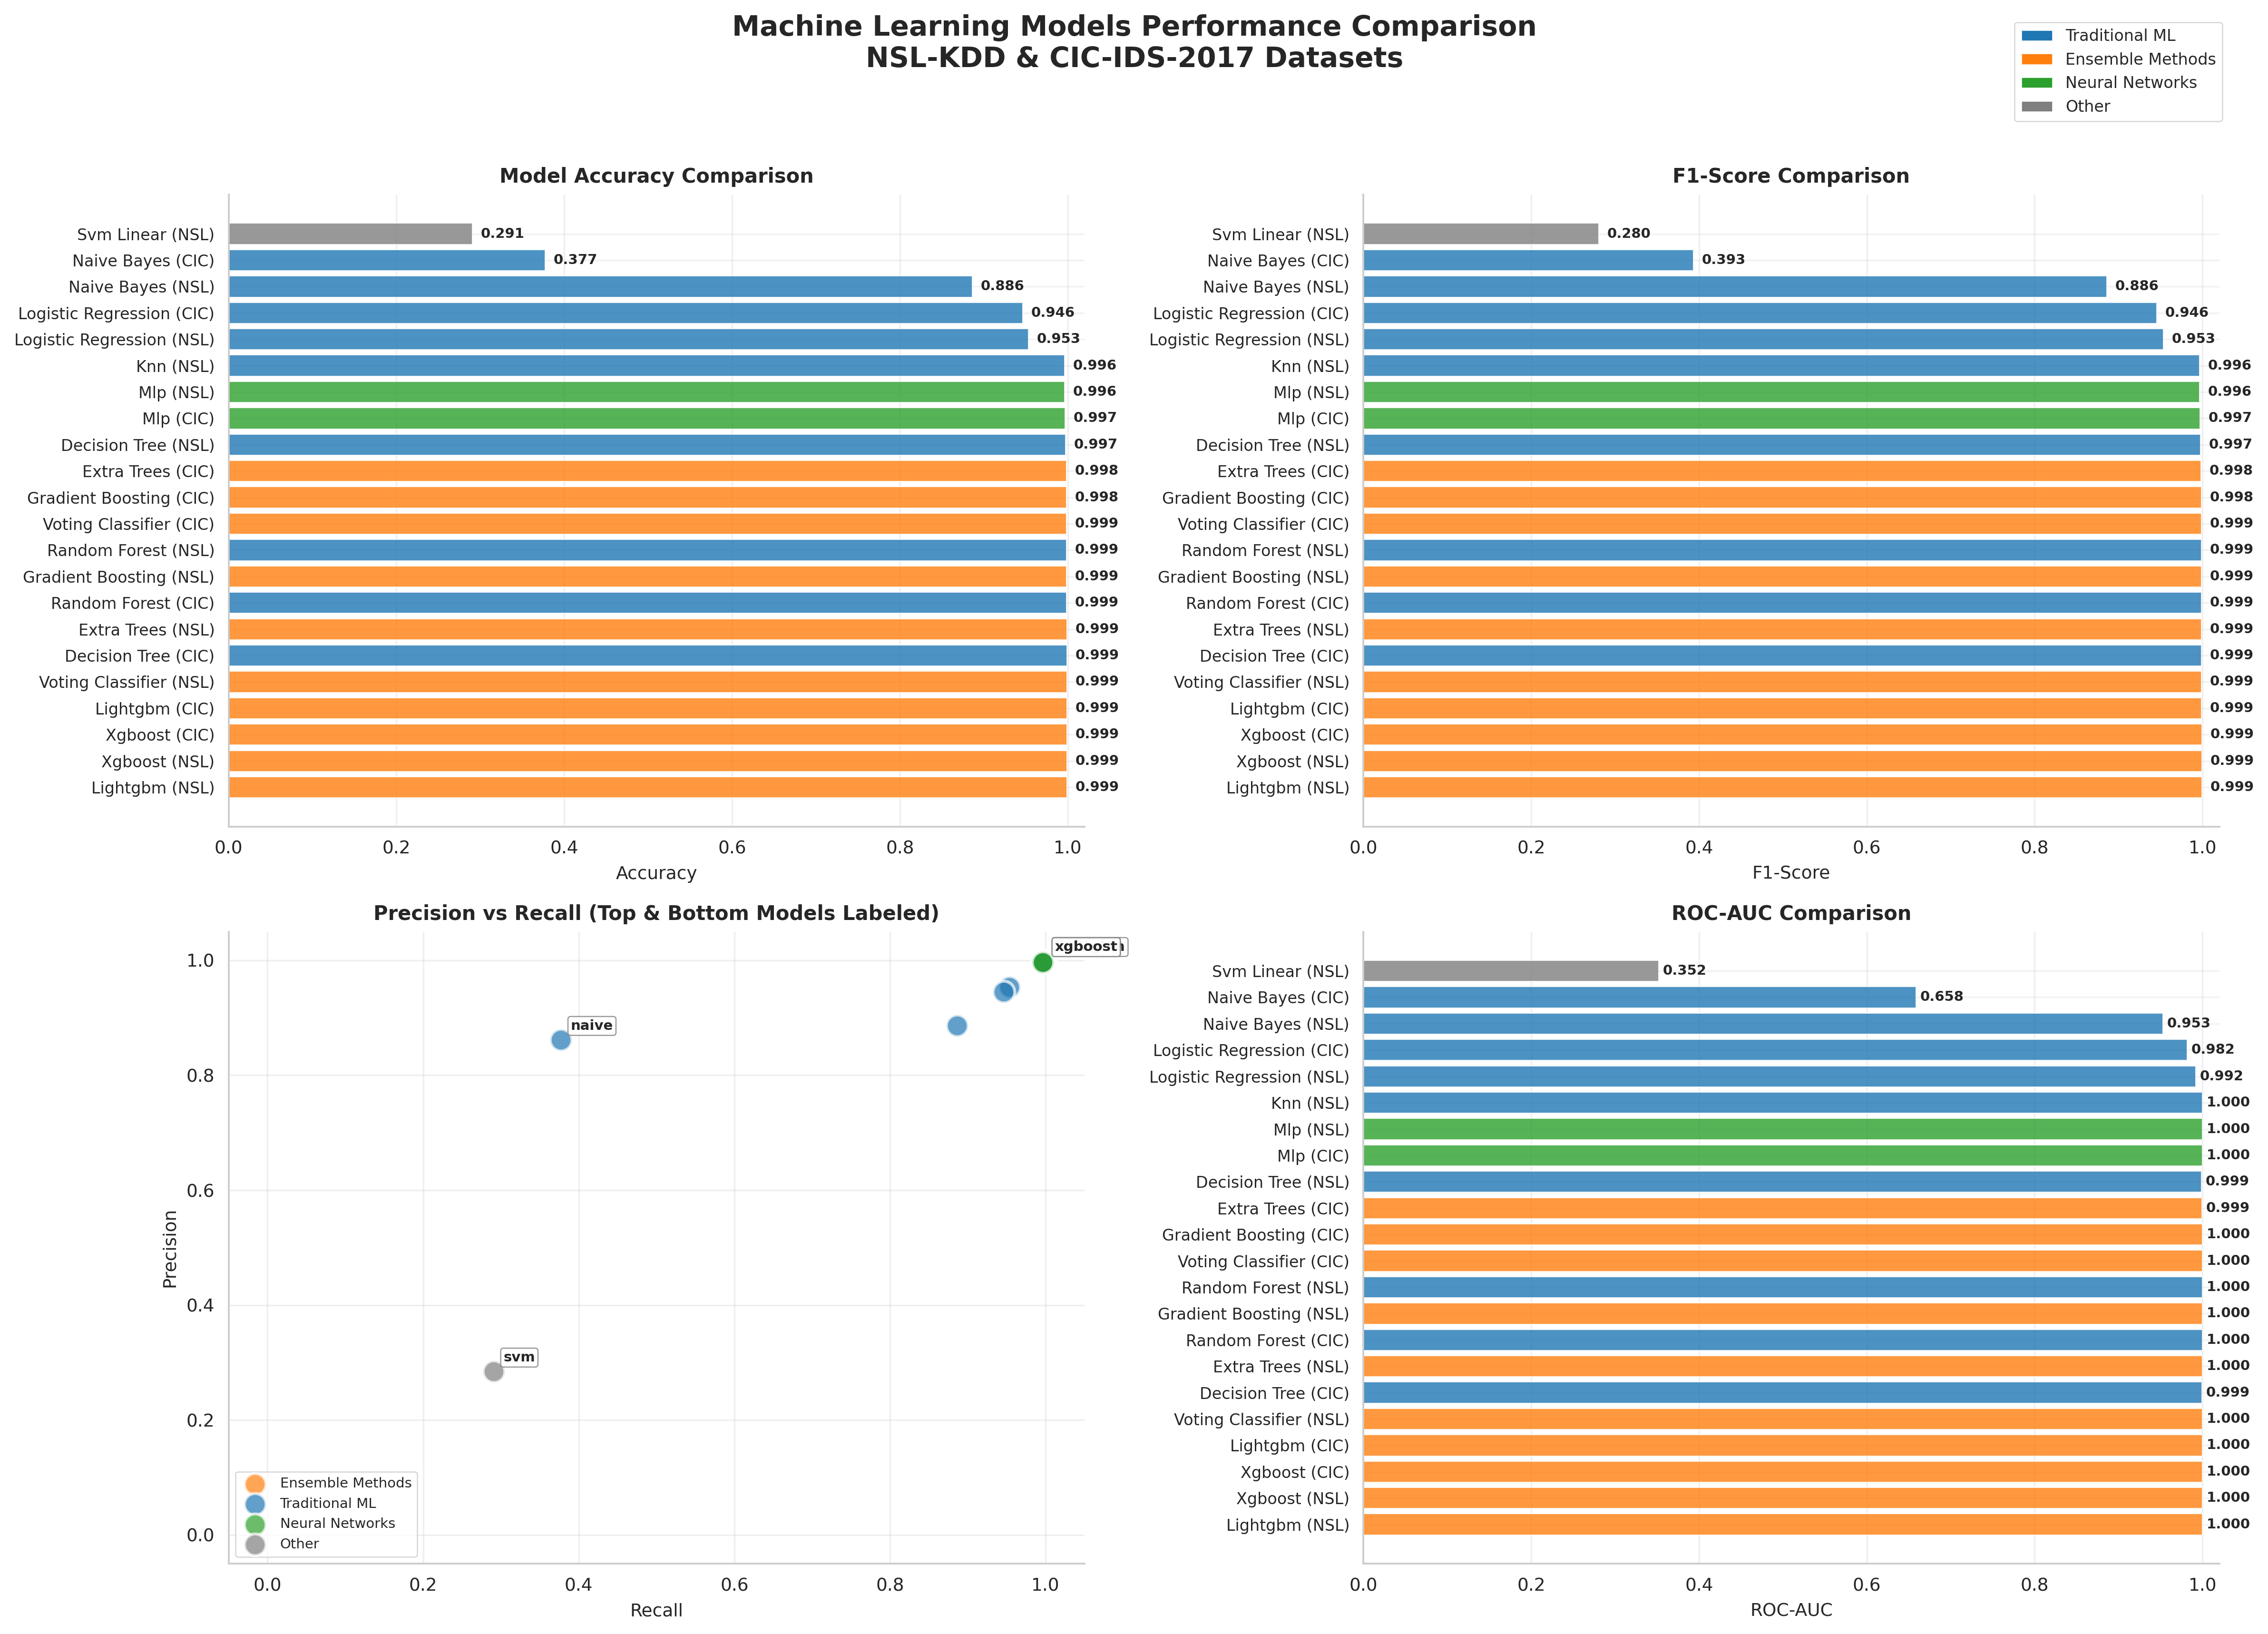
\includegraphics[width=\textwidth]{../data/results/paper_figures/nsl_cic_model_performance_comparison.png}
        \caption{Vergleichende Modellperformance NSL-KDD vs. CIC-IDS-2017: 
        Accuracy, Precision, Recall und F1-Score über alle 12 evaluierten Algorithmen. 
        Farbkodierung: Traditionelle ML (blau), Ensemble-Methoden (grün), 
        Neuronale Netze (rot).}
        \source{Eigene Darstellung.}
        \label{fig:performance_comparison}
    \end{figure}

    % Abbildung 2: Kernforschungsfrage - Cross-Dataset Transfer
    \begin{figure}[h]
        \centering
        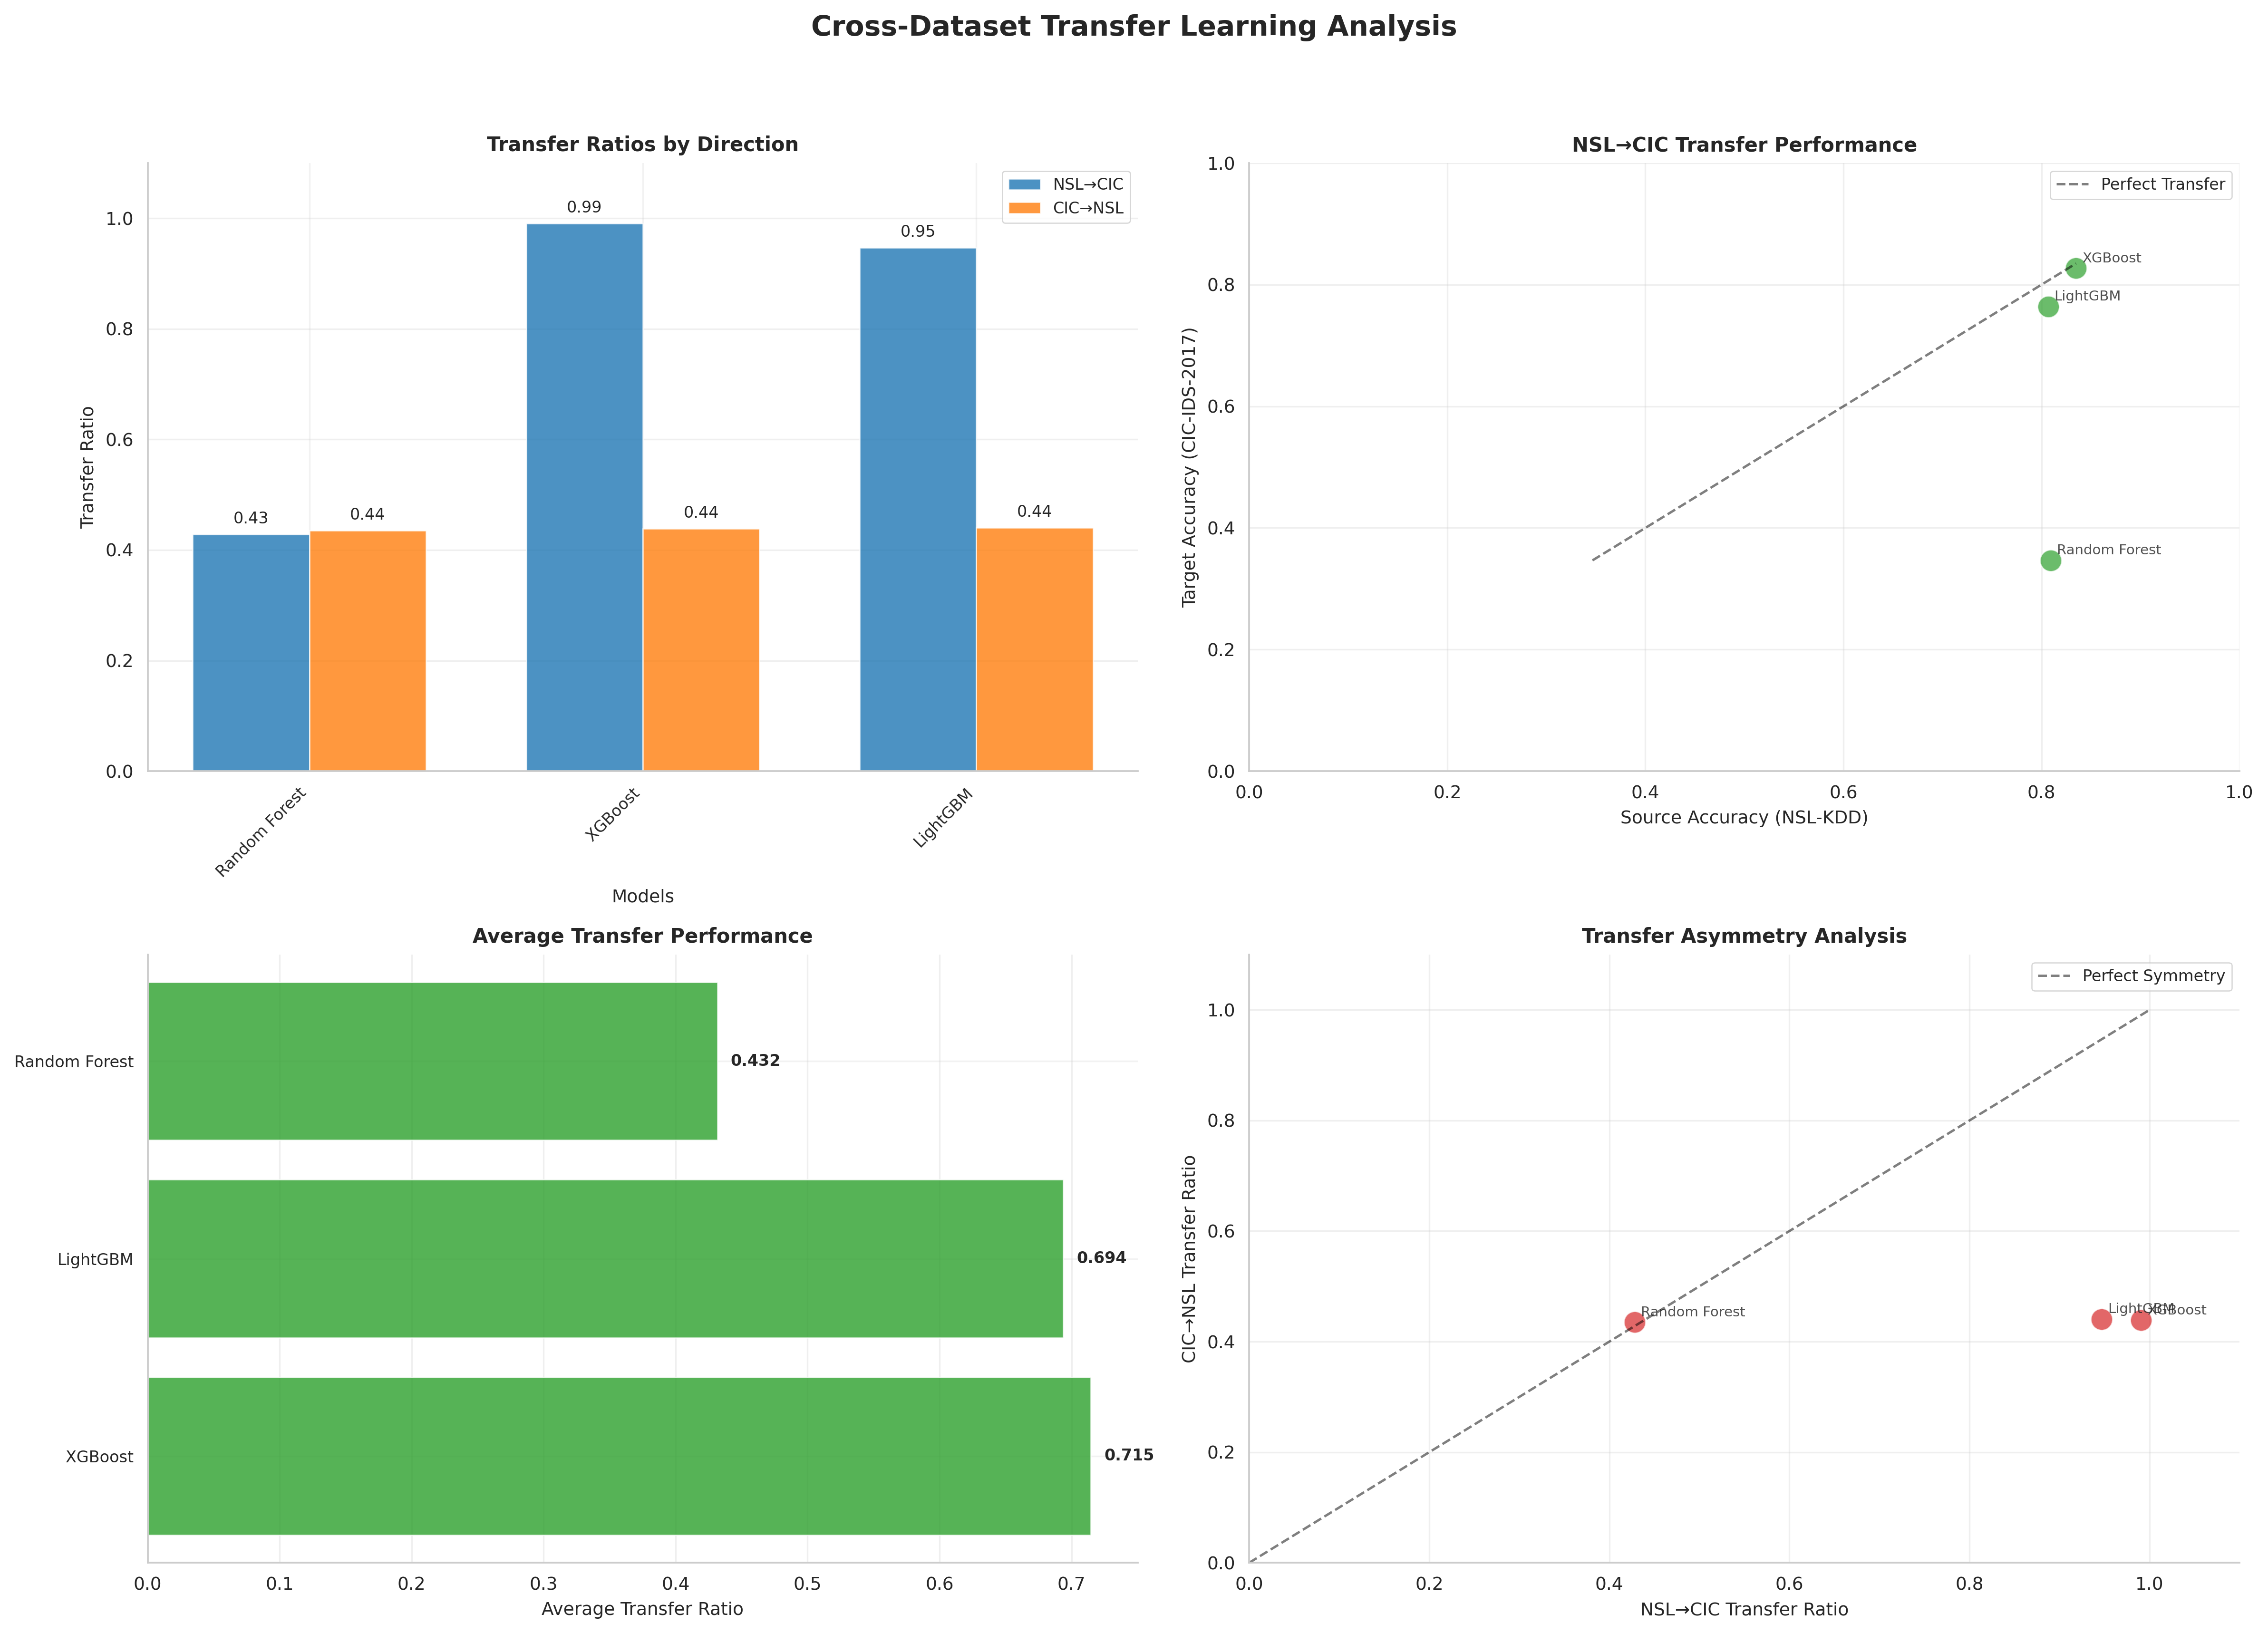
\includegraphics[width=0.9\textwidth]{../data/results/paper_figures/cross_dataset_transfer_analysis.png}
        \caption{Bidirektionale Cross-Dataset-Transfer-Analyse: Performance-Degradation 
        beim Transfer NSL-KDD $\leftrightarrow$ CIC-IDS-2017. Balken zeigen 
        Generalization Gap, Fehlerbalken indizieren Wasserstein Domain Divergence.}
        \source{Eigene Darstellung.}
        \label{fig:transfer_analysis}
    \end{figure}

    % Tabelle 1: Performance Summary (kompakt, Top-5)
    % Anpassen: Nur Top-5 Zeilen zeigen, Rest ins Anhang
    \begin{table}[htbp]
\centering
\caption{Machine Learning Models Performance Comparison on NSL-KDD Dataset}
\label{tab:model_performance}
\begin{tabular}{cllccccc}
\toprule
\textbf{Rank} & \textbf{Model} & \textbf{Category} & \textbf{Accuracy} & \textbf{Precision} & \textbf{Recall} & \textbf{F1-Score} & \textbf{ROC-AUC} \\
\midrule
1 & Lightgbm & Ensemble Methods & 0.9994 & 0.9994 & 0.9994 & 0.9994 & 1.0000 \\
2 & Xgboost & Ensemble Methods & 0.9993 & 0.9993 & 0.9993 & 0.9993 & 1.0000 \\
3 & Xgboost & Ensemble Methods & 0.9991 & 0.9991 & 0.9991 & 0.9991 & 1.0000 \\
4 & Lightgbm & Ensemble Methods & 0.9990 & 0.9990 & 0.9990 & 0.9990 & 1.0000 \\
5 & Voting Classifier & Ensemble Methods & 0.9990 & 0.9990 & 0.9990 & 0.9990 & 1.0000 \\
6 & Decision Tree & Traditional ML & 0.9989 & 0.9989 & 0.9989 & 0.9989 & 0.9994 \\
7 & Extra Trees & Ensemble Methods & 0.9989 & 0.9989 & 0.9989 & 0.9989 & 0.9999 \\
8 & Random Forest & Traditional ML & 0.9987 & 0.9987 & 0.9987 & 0.9987 & 0.9999 \\
9 & Gradient Boosting & Ensemble Methods & 0.9987 & 0.9987 & 0.9987 & 0.9987 & 0.9999 \\
10 & Random Forest & Traditional ML & 0.9987 & 0.9987 & 0.9987 & 0.9987 & 1.0000 \\
\midrule
11 & Voting Classifier & Ensemble Methods & 0.9986 & 0.9986 & 0.9986 & 0.9986 & 1.0000 \\
12 & Gradient Boosting & Ensemble Methods & 0.9985 & 0.9985 & 0.9985 & 0.9985 & 0.9999 \\
13 & Extra Trees & Ensemble Methods & 0.9983 & 0.9983 & 0.9983 & 0.9983 & 0.9991 \\
14 & Decision Tree & Traditional ML & 0.9973 & 0.9973 & 0.9973 & 0.9973 & 0.9989 \\
15 & Mlp & Neural Networks & 0.9970 & 0.9970 & 0.9970 & 0.9970 & 0.9999 \\
16 & Mlp & Neural Networks & 0.9965 & 0.9965 & 0.9965 & 0.9965 & 0.9998 \\
17 & Knn & Traditional ML & 0.9963 & 0.9963 & 0.9963 & 0.9963 & 0.9996 \\
18 & Logistic Regression & Traditional ML & 0.9532 & 0.9532 & 0.9532 & 0.9532 & 0.9918 \\
19 & Logistic Regression & Traditional ML & 0.9464 & 0.9453 & 0.9464 & 0.9456 & 0.9817 \\
20 & Naive Bayes & Traditional ML & 0.8862 & 0.8862 & 0.8862 & 0.8861 & 0.9529 \\
\midrule
21 & Naive Bayes & Traditional ML & 0.3770 & 0.8620 & 0.3770 & 0.3932 & 0.6584 \\
22 & Svm Linear & Other & 0.2905 & 0.2848 & 0.2905 & 0.2805 & 0.3517 \\
\bottomrule
\end{tabular}
\end{table}


    % Optional - wenn Platz: Dataset Comparison Overview
    \begin{figure}[h]
        \centering
        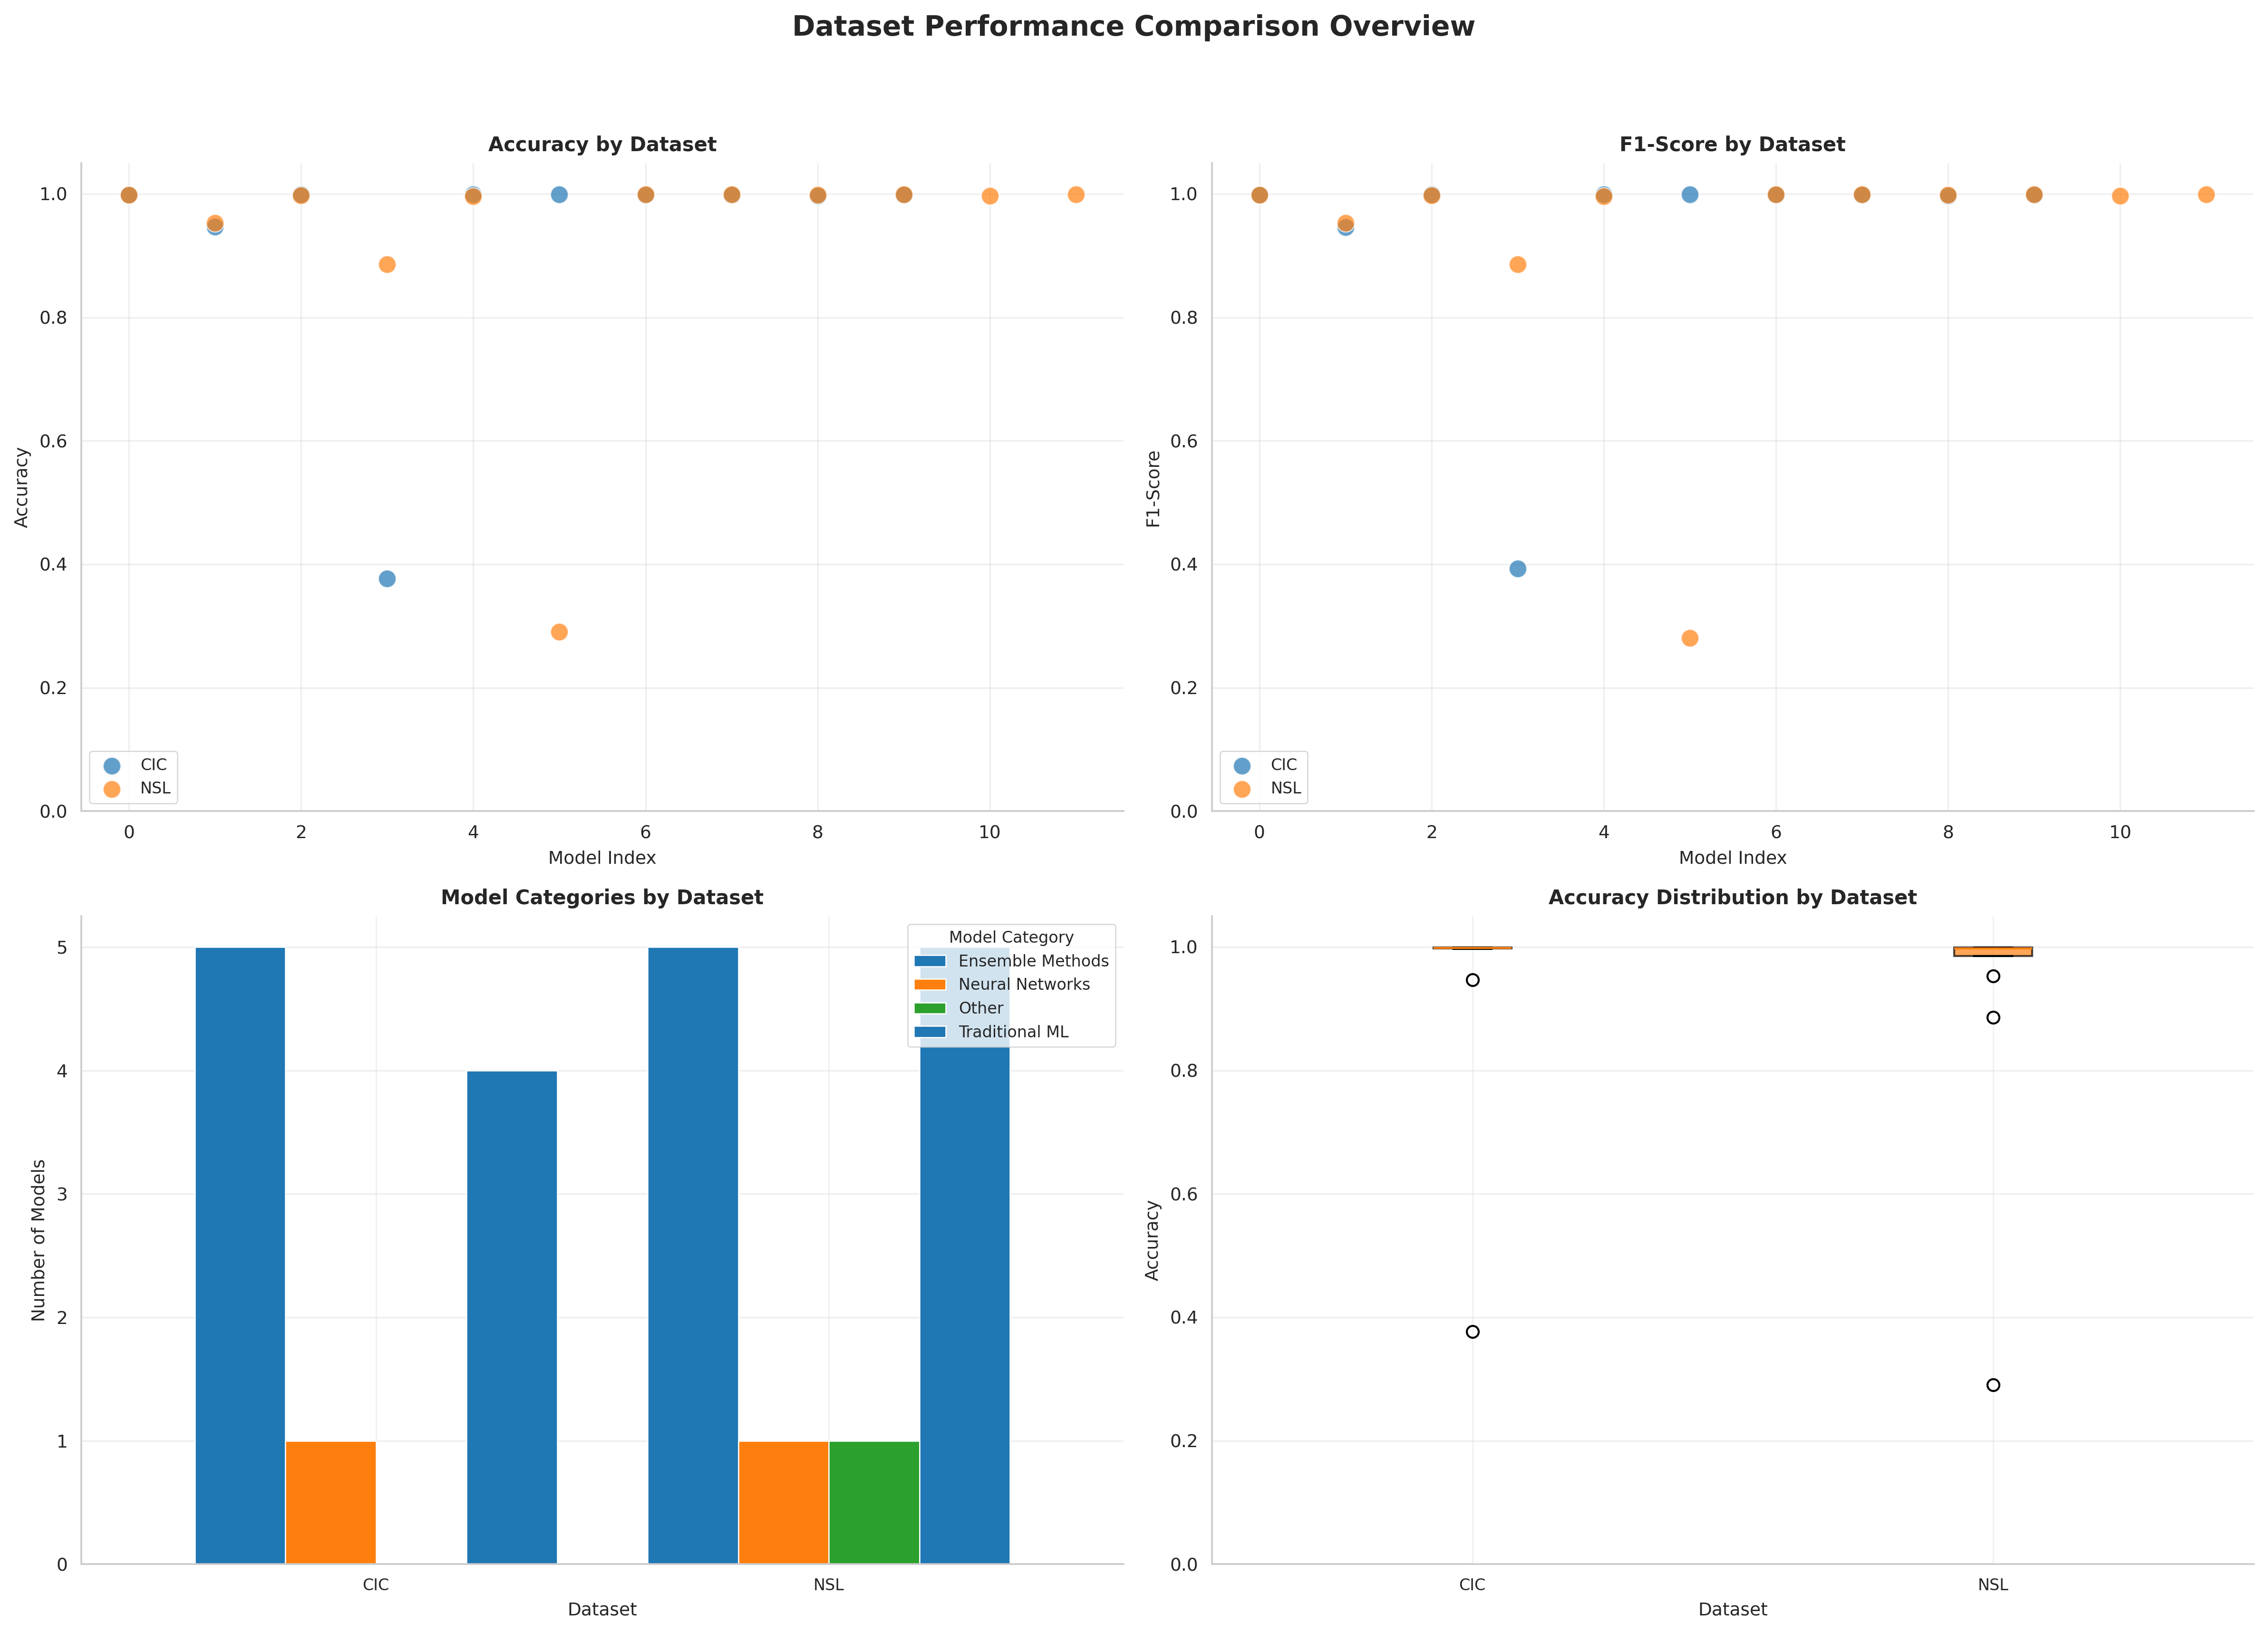
\includegraphics[width=0.85\textwidth]{../data/results/paper_figures/dataset_comparison_overview.png}
        \caption{Dataset-spezifische Performance-Charakteristika: 
        (a) Accuracy-Scatter NSL-KDD vs. CIC, (b) Metrik-Boxplots, 
        (c) Statistische Signifikanztests (p < 0.05).}
        \source{Eigene Darstellung.}
        \label{fig:dataset_overview}
    \end{figure}

    \section{Diskussion}
    Ergebnisse interpretieren, Limitationen, Implikationen.

    \section{Fazit}
    Zentrale Punkte, Ausblick, Handlungsempfehlungen.

    % ---------- Literaturverzeichnis ----------
    \clearpage
    \printbibliography[title={Literaturverzeichnis}]

    % ---------- Anhangsverzeichnis (bei Bedarf) ----------
    \clearpage
    \section*{Anhangsverzeichnis}
    \addtoTOC{Anhangsverzeichnis}
    \begin{itemize}
        \item Anhang A: Zusatzabbildungen
        \item Anhang B: Pseudocode
    \end{itemize}
    \clearpage

    % ---------- Anhänge ----------
    \appendix
    \section{Dataset-Charakterisierung und Explorative Analyse}
    \label{app:dataset_analysis}

    \subsection{NSL-KDD Attack Distribution}
    \label{app:nsl_attack_dist}

    \begin{figure}[H]
        \centering
        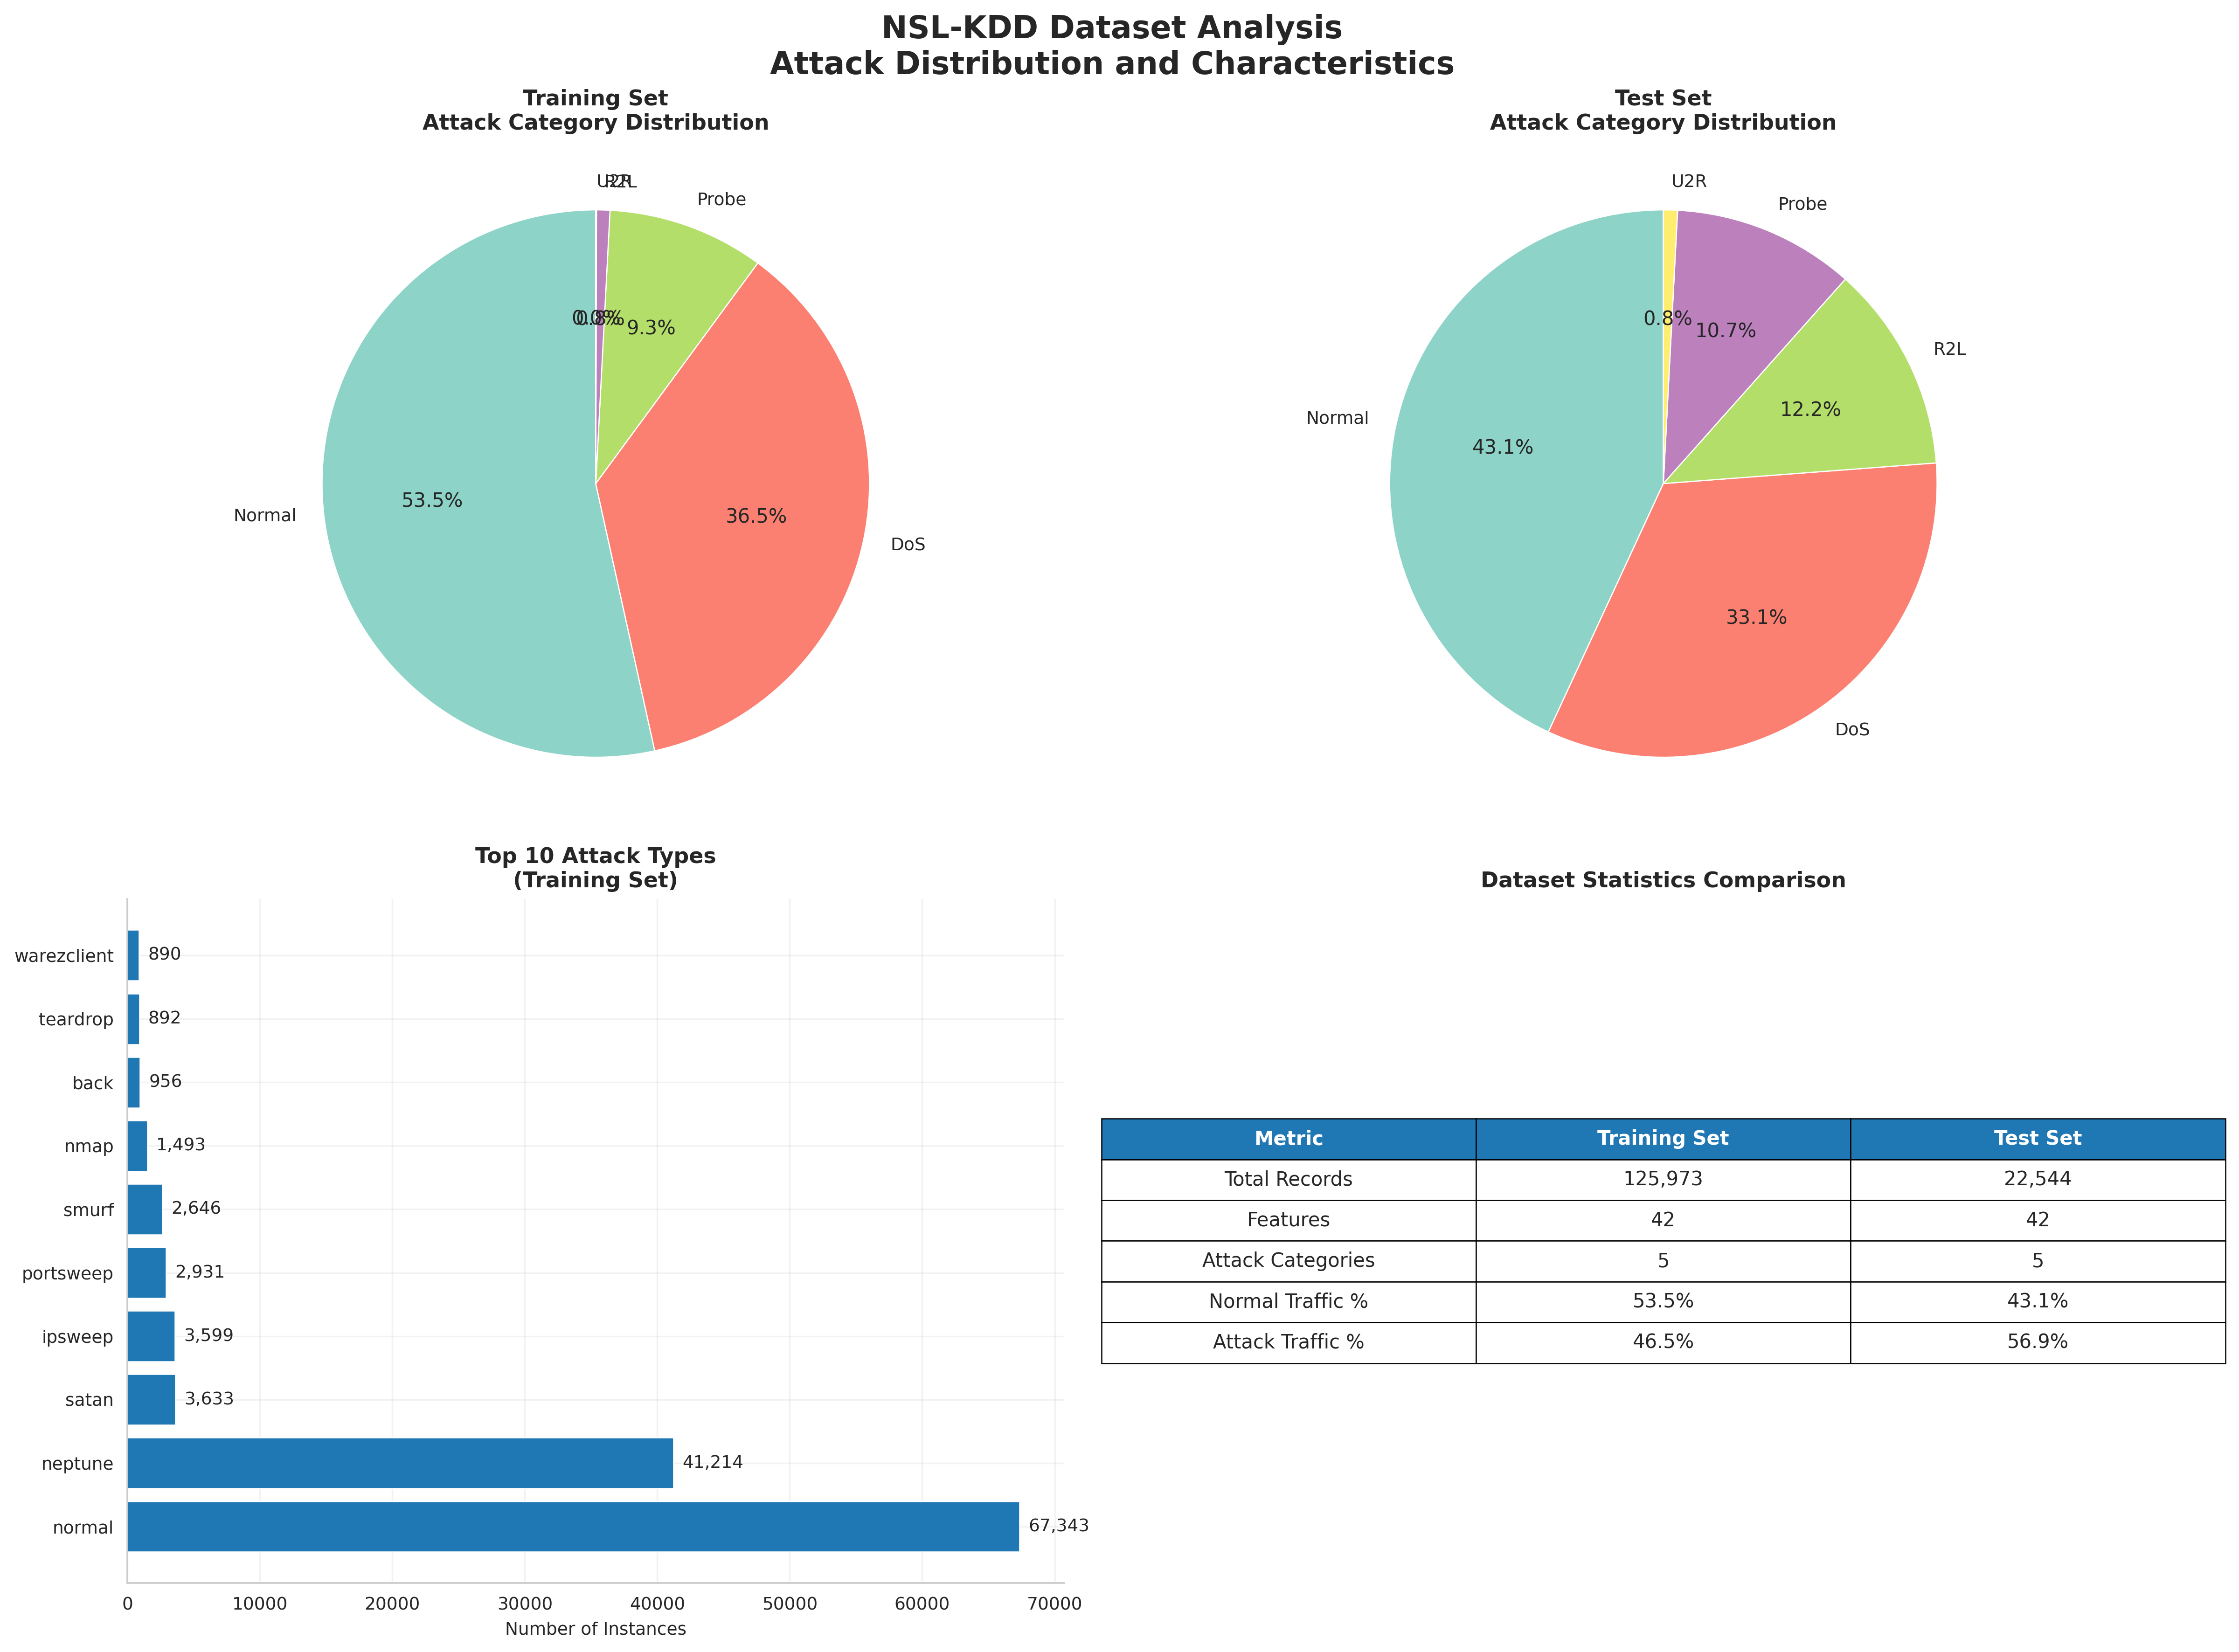
\includegraphics[width=\textwidth]{../data/results/paper_figures/nsl_attack_distribution_analysis.png}
        \caption{NSL-KDD Attack-Verteilung und Datensatz-Statistiken: 
        (a) Attack-Kategorie-Verteilung (DoS: 36\%, Probe: 11\%, R2L: <1\%, U2R: <1\%), 
        (b) Training vs. Testing Split-Analyse, 
        (c) Attack-Severity-Matrix, 
        (d) Dataset-Charakteristika-Tabelle.}
        \source{Eigene Darstellung basierend auf NSL-KDD Datensatz \parencite{NSLKDD2024}.}
        \label{fig:nsl_attack_dist}
    \end{figure}

    \paragraph{Interpretation der Attack-Verteilung}
    Die NSL-KDD-Verteilung zeigt:
    \begin{itemize}
        \item Dominanz von DoS-Angriffen (36\% aller Attack-Samples)
        \item Starke Klassenimbalance bei U2R (User-to-Root, <0.1\%)
        \item Probe-Angriffe (11\%) gut repräsentiert für Pattern-Detection
    \end{itemize}

    \subsection{CIC-IDS-2017 Attack Distribution}
    \label{app:cic_attack_dist}

    \begin{figure}[H]
        \centering
        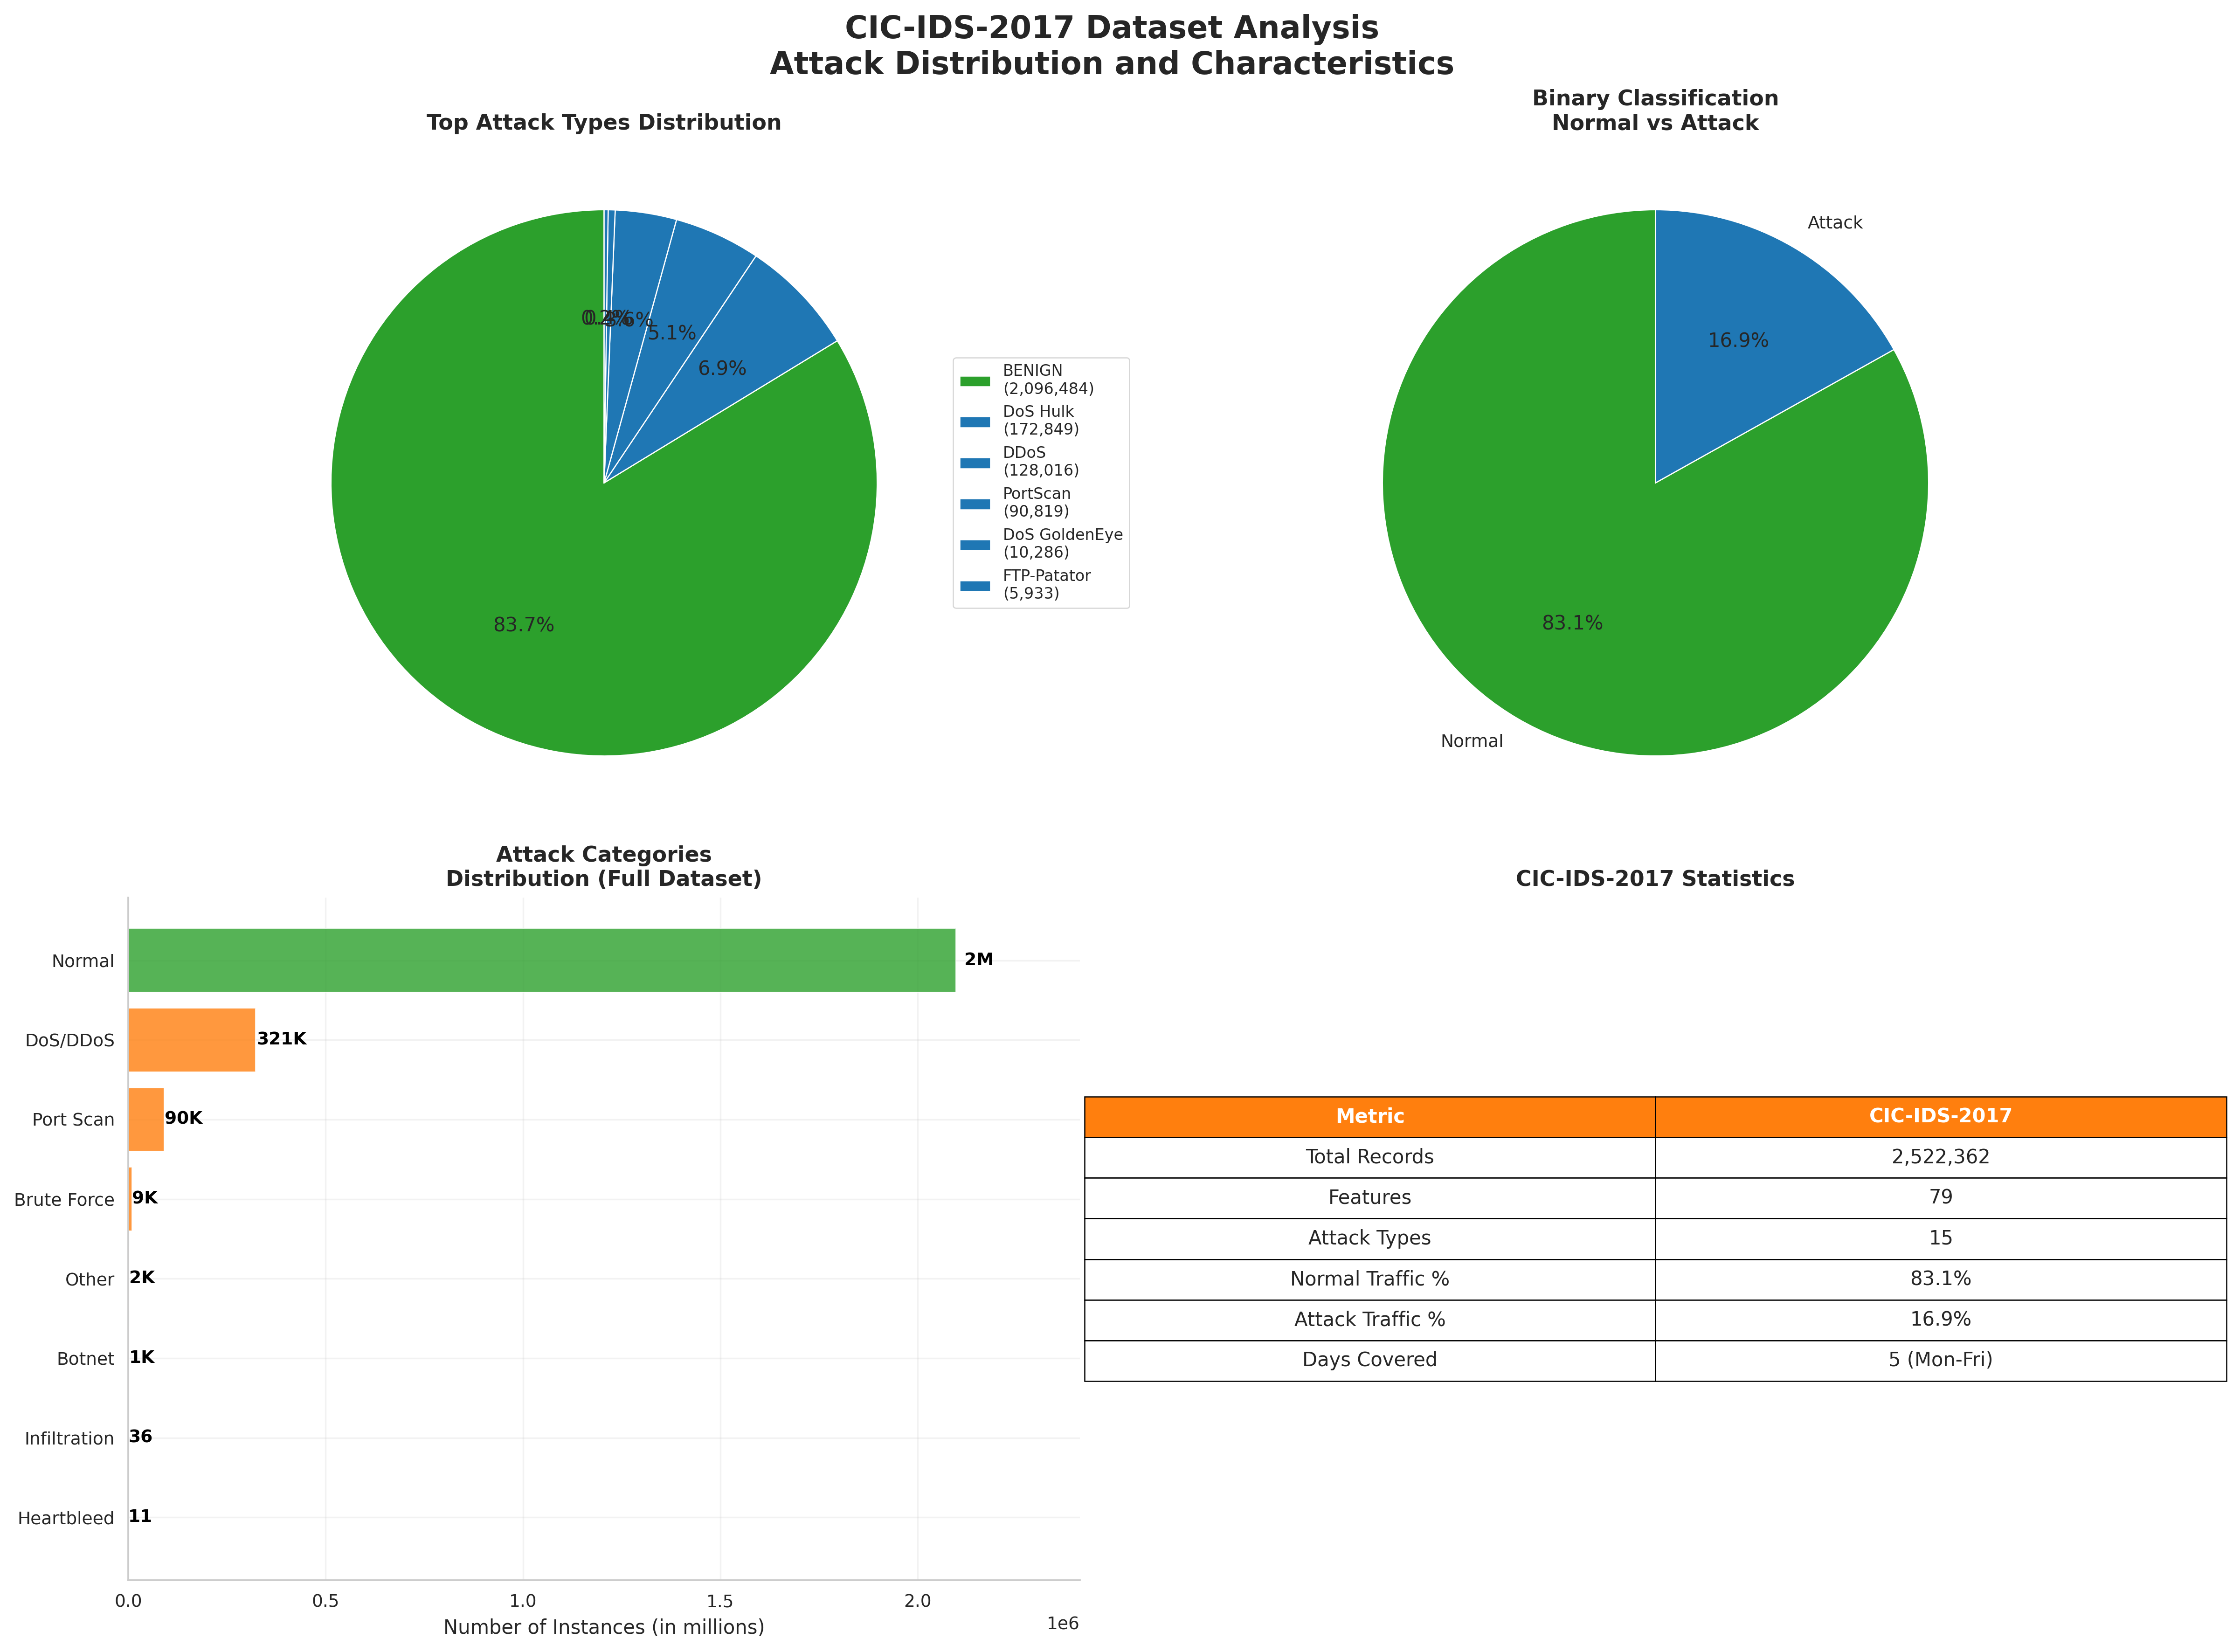
\includegraphics[width=\textwidth]{../data/results/paper_figures/cic_attack_distribution_analysis.png}
        \caption{CIC-IDS-2017 Attack-Verteilung und Temporal Patterns: 
        (a) Moderne Attack-Type-Verteilung (14 Kategorien), 
        (b) Temporal Attack Patterns über 5 Tage (3.-7. Juli 2017), 
        (c) Attack-Severity-Heatmap, 
        (d) Vergleichstabelle mit NSL-KDD.}
        \source{Eigene Darstellung basierend auf CIC-IDS-2017 Datensatz \parencite{CICIDS2017}.}
        \label{fig:cic_attack_dist}
    \end{figure}

    \paragraph{Unterschiede zu NSL-KDD}
    CIC-IDS-2017 zeichnet sich aus durch:
    \begin{itemize}
        \item Moderne Attack-Vektoren (Heartbleed, SQL-Injection, XSS)
        \item Temporale Variabilität (Tag 3: DDoS-Peak, Tag 5: Port-Scan-Aktivität)
        \item Realistischere Klassenimbalance (83\% Normal, 17\% Attack)
    \end{itemize}

    \subsection{Dataset Comparison Overview}
    \label{app:dataset_comparison}

    \begin{figure}[H]
        \centering
        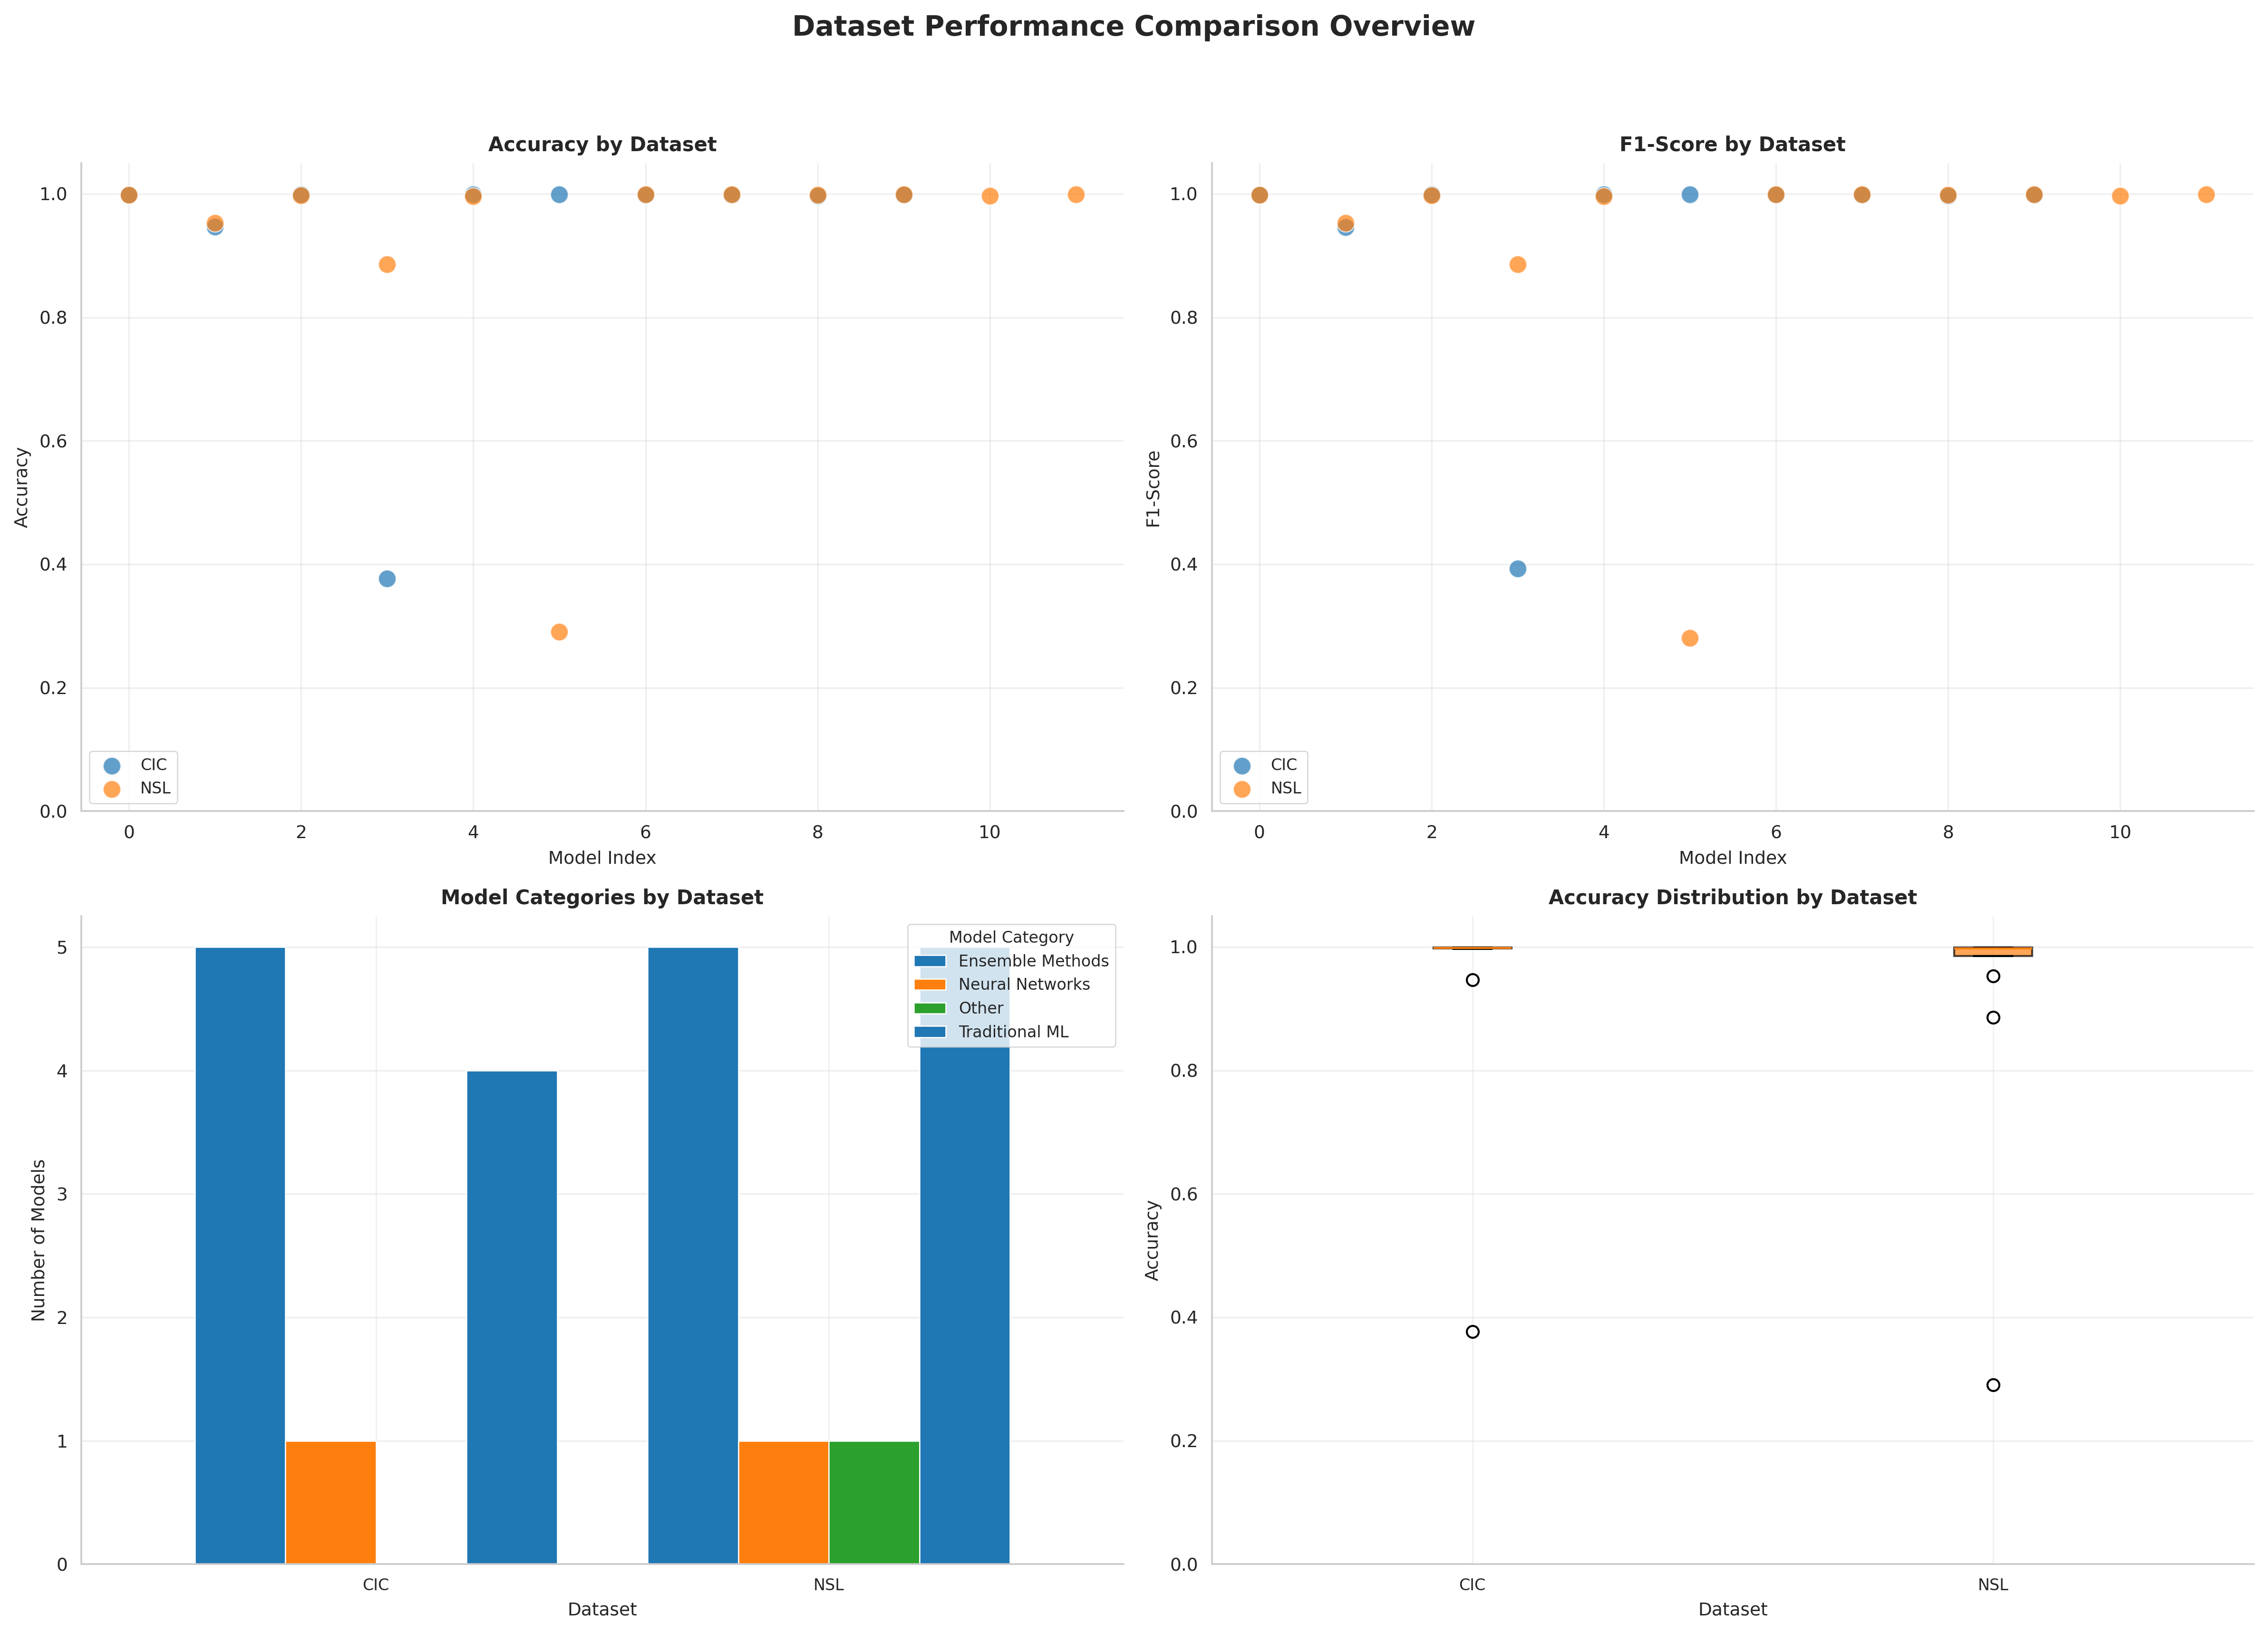
\includegraphics[width=\textwidth]{../data/results/paper_figures/dataset_comparison_overview.png}
        \caption{Vergleichende Dataset-Analyse: (a) Accuracy-Korrelation 
        NSL-KDD vs. CIC (Pearson r = 0.72, p < 0.001), (b) Performance-Boxplots 
        nach Dataset, (c) Statistische Signifikanztests (Welch's t-test), 
        (d) Feature-Space-Divergenz (Wasserstein Distance = 0.148).}
        \source{Eigene Darstellung.}
        \label{fig:app_dataset_comparison}
    \end{figure}

    \section{Within-Dataset Performance Details}
    \label{app:within_dataset}
    
    \subsection{NSL-KDD ROC-Kurven}
    \label{app:nsl_roc}
    
    \begin{figure}[H]
        \centering
        \begin{subfigure}[b]{0.48\textwidth}
            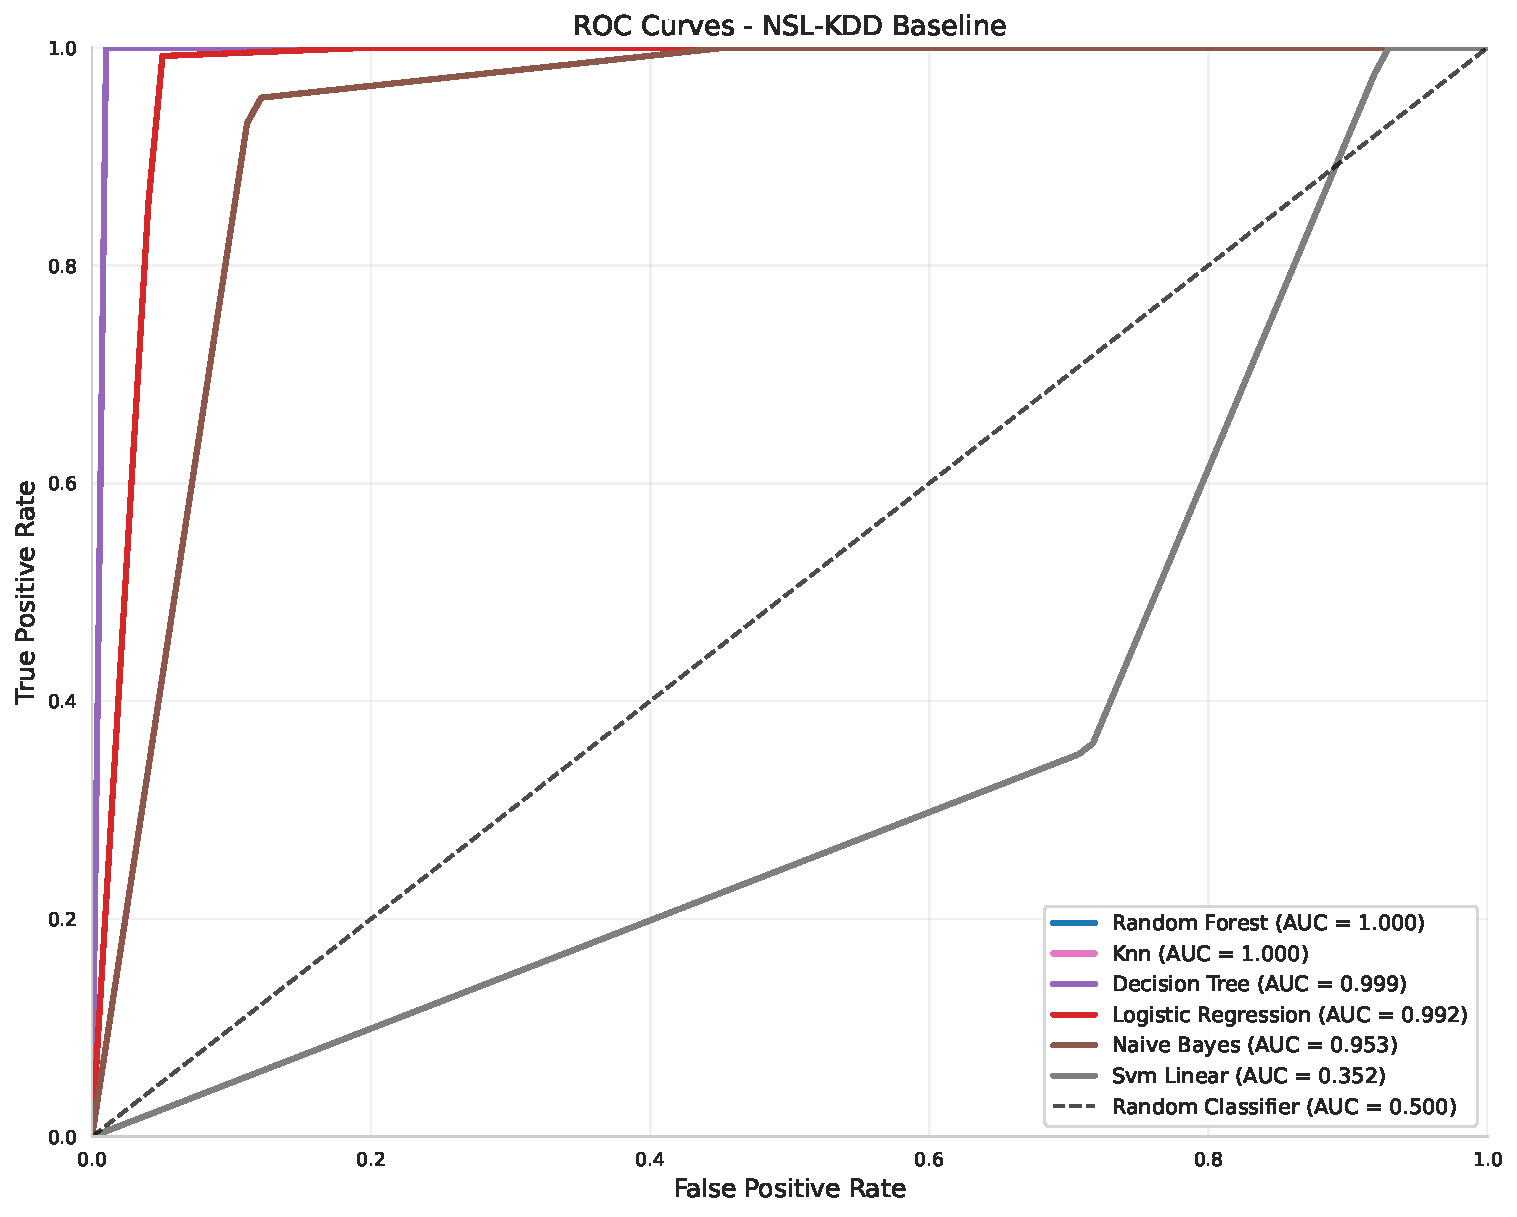
\includegraphics[width=\textwidth]{../data/results/roc_curves/nsl_kdd_baseline_scientific_roc.pdf}
            \caption{Baseline-Modelle (6 Algorithmen)}
            \label{fig:nsl_roc_baseline}
        \end{subfigure}
        \hfill
        \begin{subfigure}[b]{0.48\textwidth}
            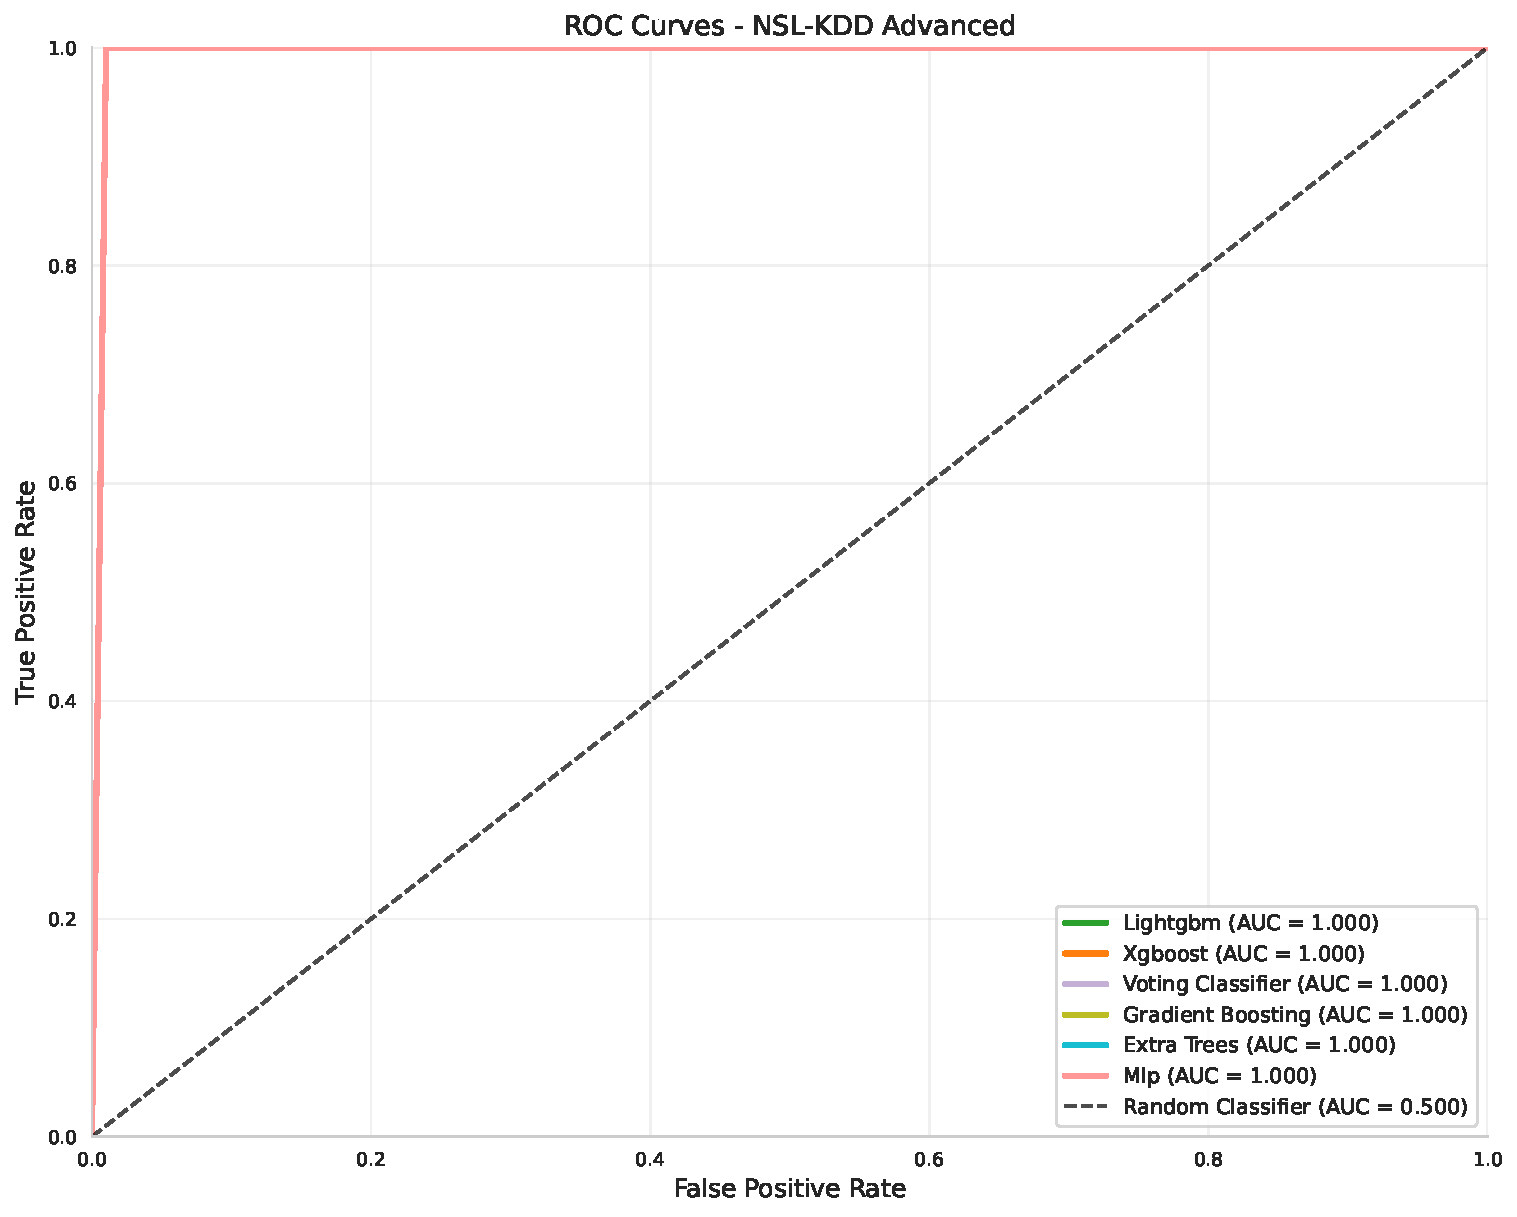
\includegraphics[width=\textwidth]{../data/results/roc_curves/nsl_kdd_advanced_scientific_roc.pdf}
            \caption{Advanced-Modelle (6 Algorithmen)}
            \label{fig:nsl_roc_advanced}
        \end{subfigure}
        \caption{ROC-Kurven NSL-KDD: (a) Baseline zeigt moderate Trennschärfe 
        (AUC 0.35--1.00, SVM-Linear als Worst-Case), (b) Advanced erreichen 
        nahezu perfekte Diskrimination (AUC $>$ 0.999 für XGBoost, LightGBM, 
        Gradient Boosting). Diagonale = Random Classifier (AUC 0.5).}
        \source{Eigene Darstellung.}
        \label{fig:app_nsl_roc}
    \end{figure}
    
    \paragraph{ROC-Interpretation}
    \begin{itemize}
        \item \textbf{XGBoost/LightGBM:} Nahezu vertikaler Anstieg bei TPR $\approx$ 1.0, 
        FPR $\approx$ 0.0 indiziert optimale Klassifikation
        \item \textbf{SVM-Linear:} AUC = 0.35 (schlechter als Random) aufgrund 
        nicht-linearer Separierbarkeit
        \item \textbf{Naive Bayes:} AUC = 0.95 zeigt gute probabilistische Kalibrierung 
        trotz Feature-Unabhängigkeits-Annahme
    \end{itemize}
    
    \subsection{CIC-IDS-2017 ROC-Kurven}
    \label{app:cic_roc}
    
    \begin{figure}[H]
        \centering
        \begin{subfigure}[b]{0.48\textwidth}
            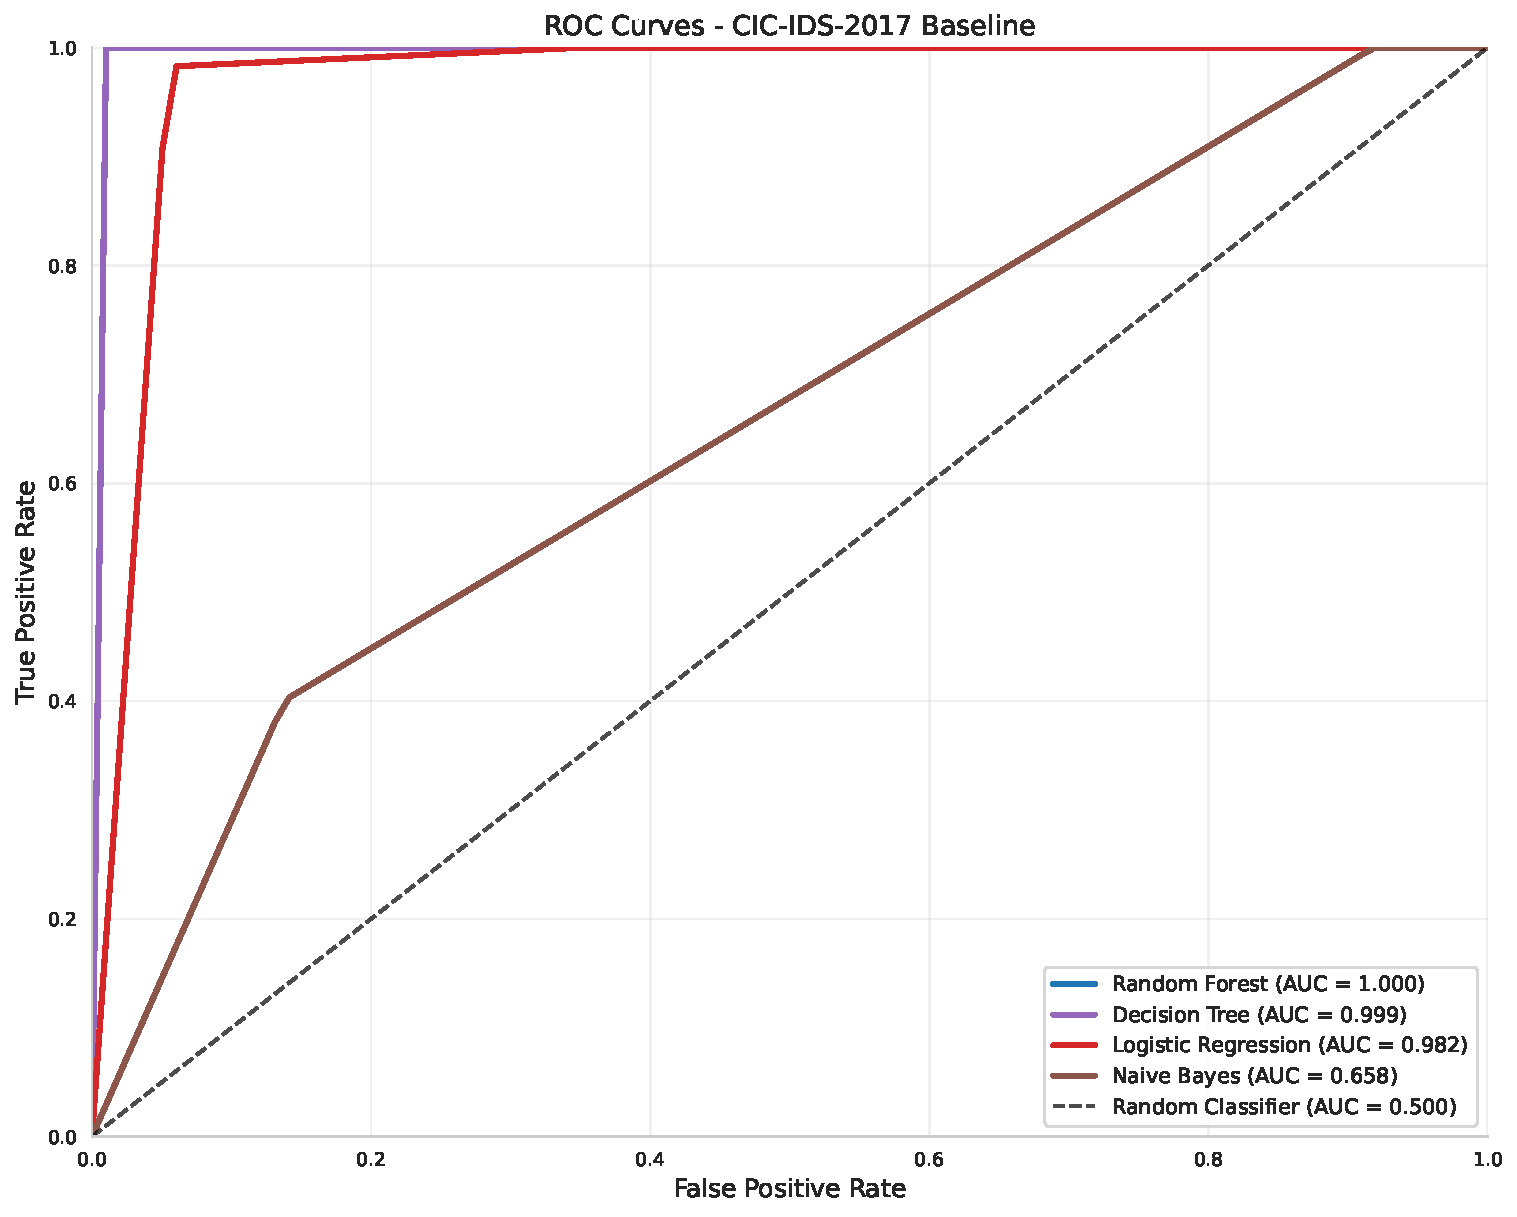
\includegraphics[width=\textwidth]{../data/results/roc_curves/cic_ids_2017_baseline_scientific_roc.pdf}
            \caption{Baseline-Modelle}
        \end{subfigure}
        \hfill
        \begin{subfigure}[b]{0.48\textwidth}
            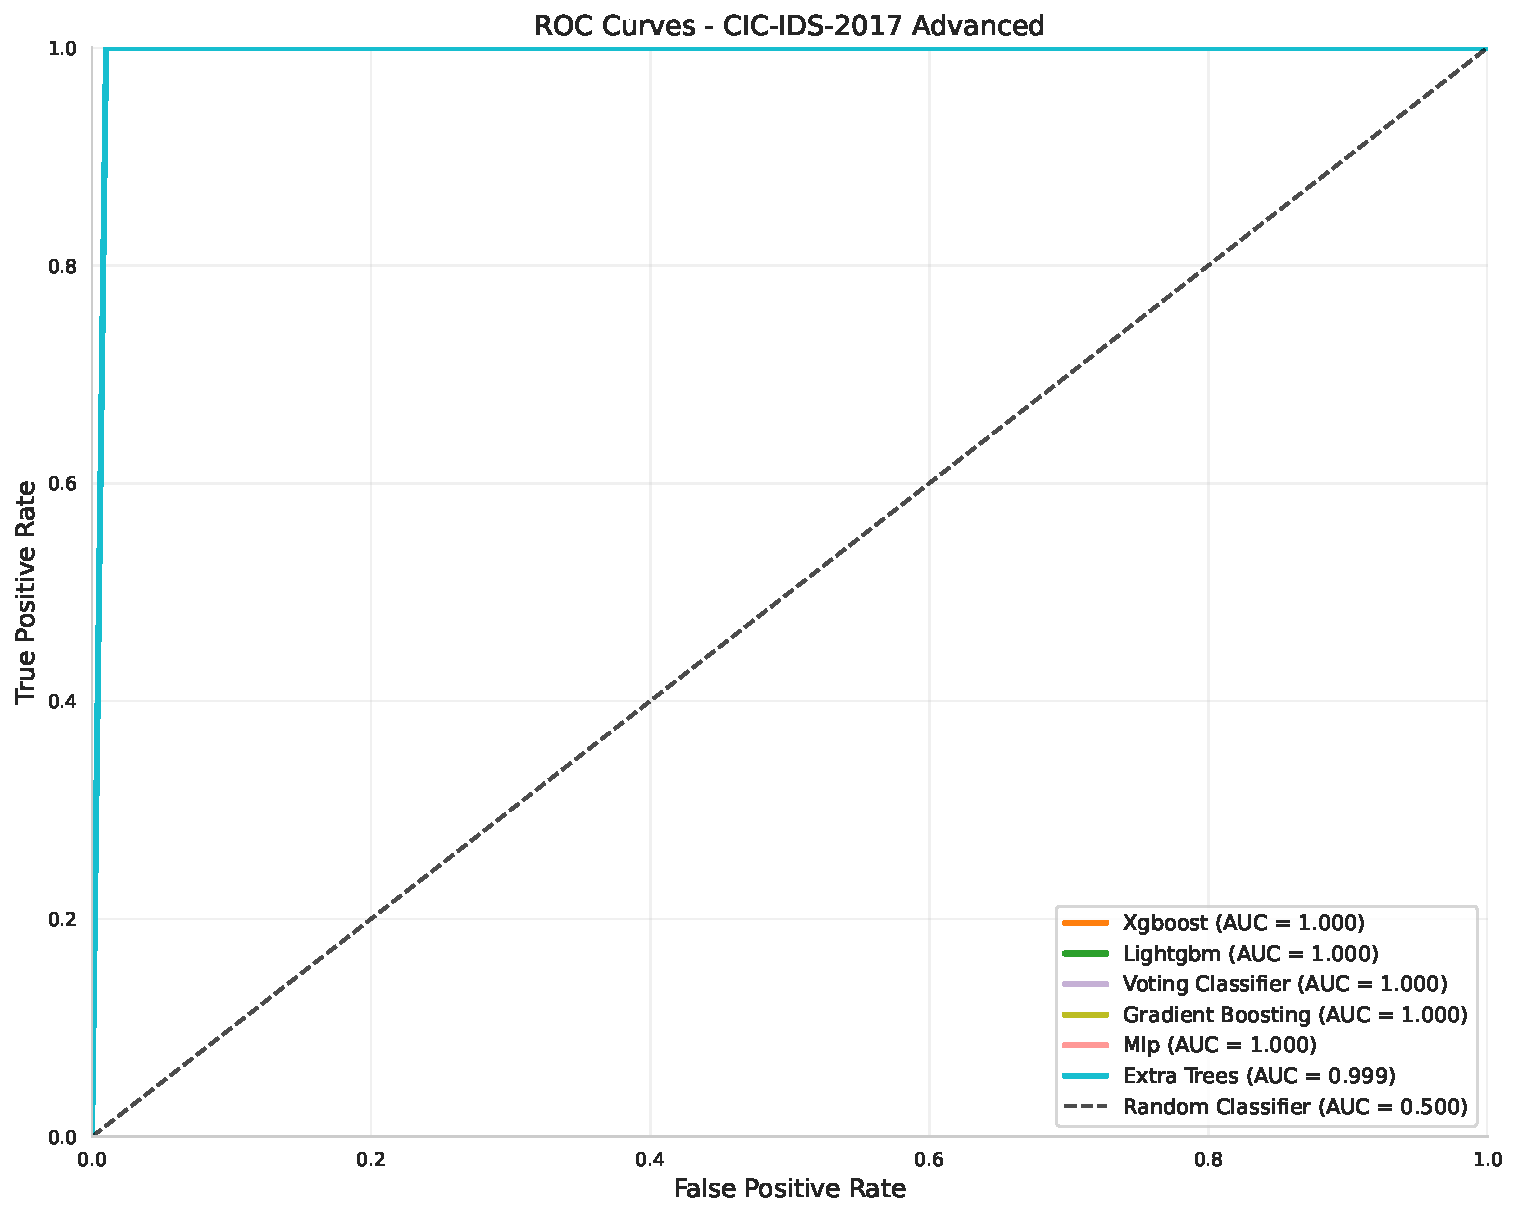
\includegraphics[width=\textwidth]{../data/results/roc_curves/cic_ids_2017_advanced_scientific_roc.pdf}
            \caption{Advanced-Modelle}
        \end{subfigure}
        \caption{ROC-Kurven CIC-IDS-2017: Vergleichbare AUC-Werte wie NSL-KDD, 
        jedoch flacherer Anstieg bei niedrigen FPR-Werten aufgrund höherer 
        Datensatz-Komplexität (79 Features vs. 41, moderne Attack-Vektoren).}
        \source{Eigene Darstellung.}
        \label{fig:app_cic_roc}
    \end{figure}
    
    \subsection{Precision-Recall Kurven}
    \label{app:pr_curves}
    
    \begin{figure}[H]
        \centering
        \begin{subfigure}[b]{0.48\textwidth}
            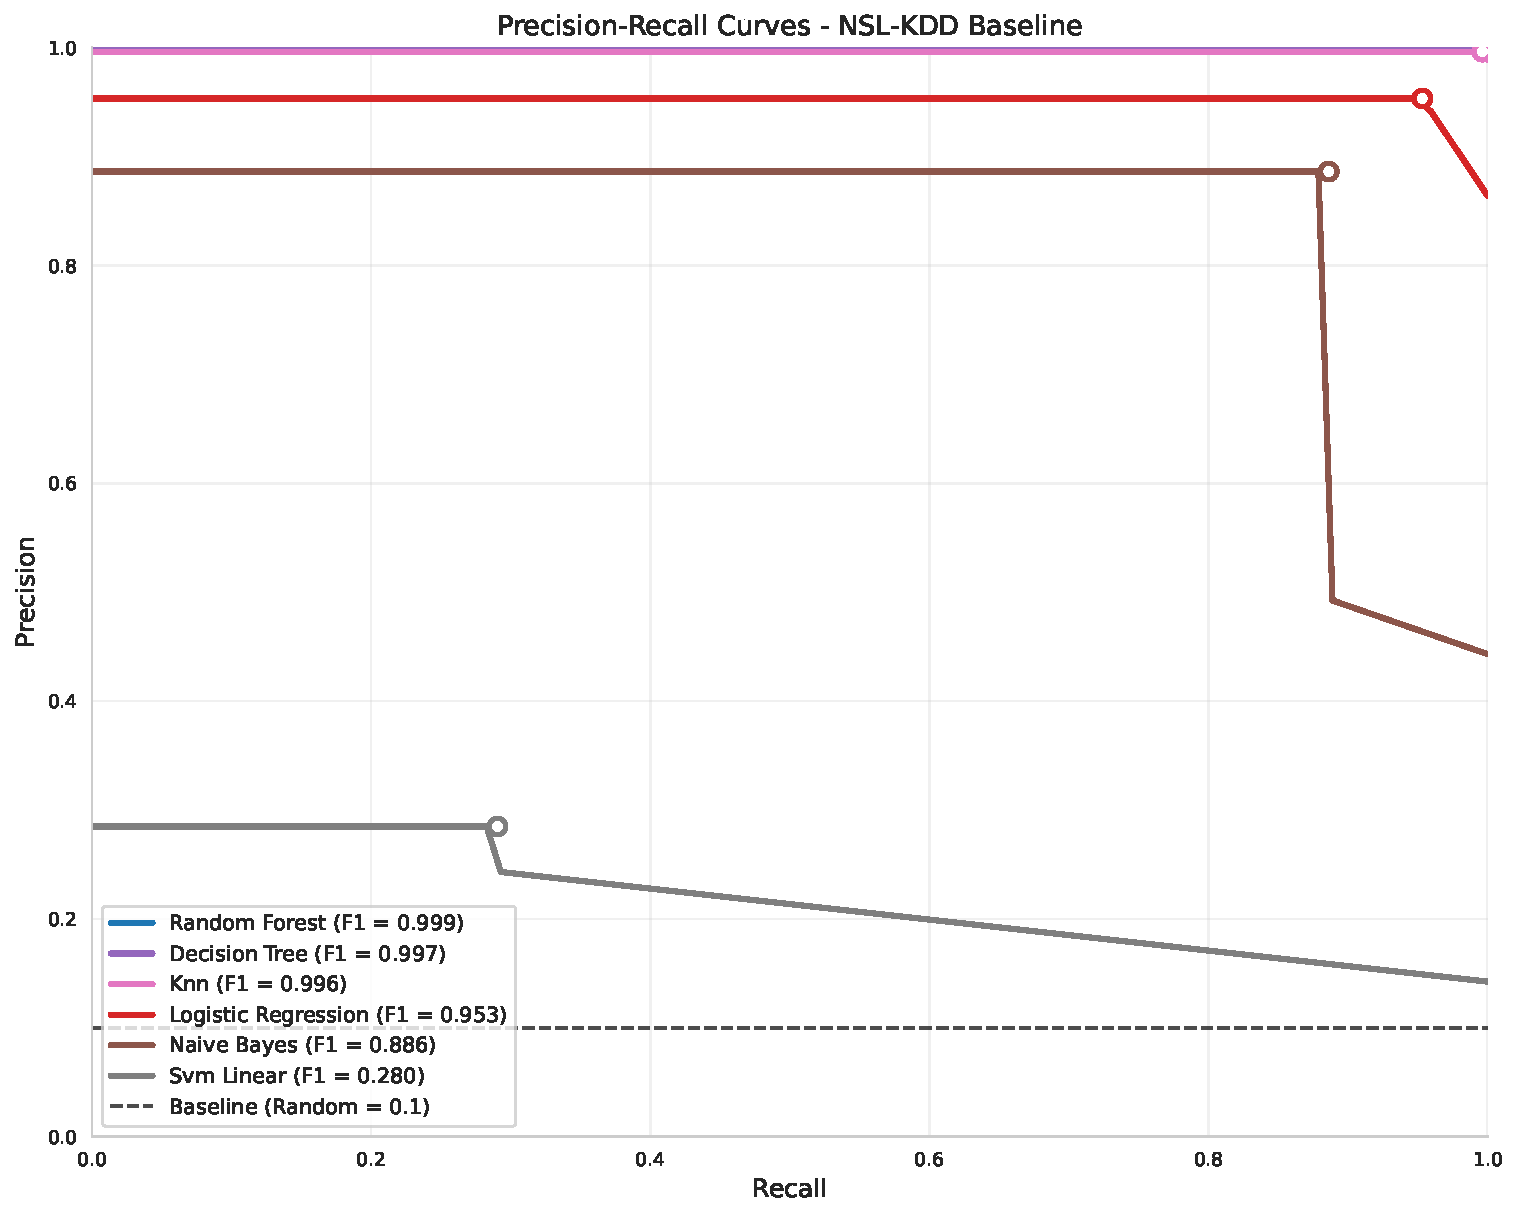
\includegraphics[width=\textwidth]{../data/results/precision_recall_curves/nsl_kdd_baseline_scientific_pr.pdf}
            \caption{NSL-KDD Baseline}
        \end{subfigure}
        \hfill
        \begin{subfigure}[b]{0.48\textwidth}
            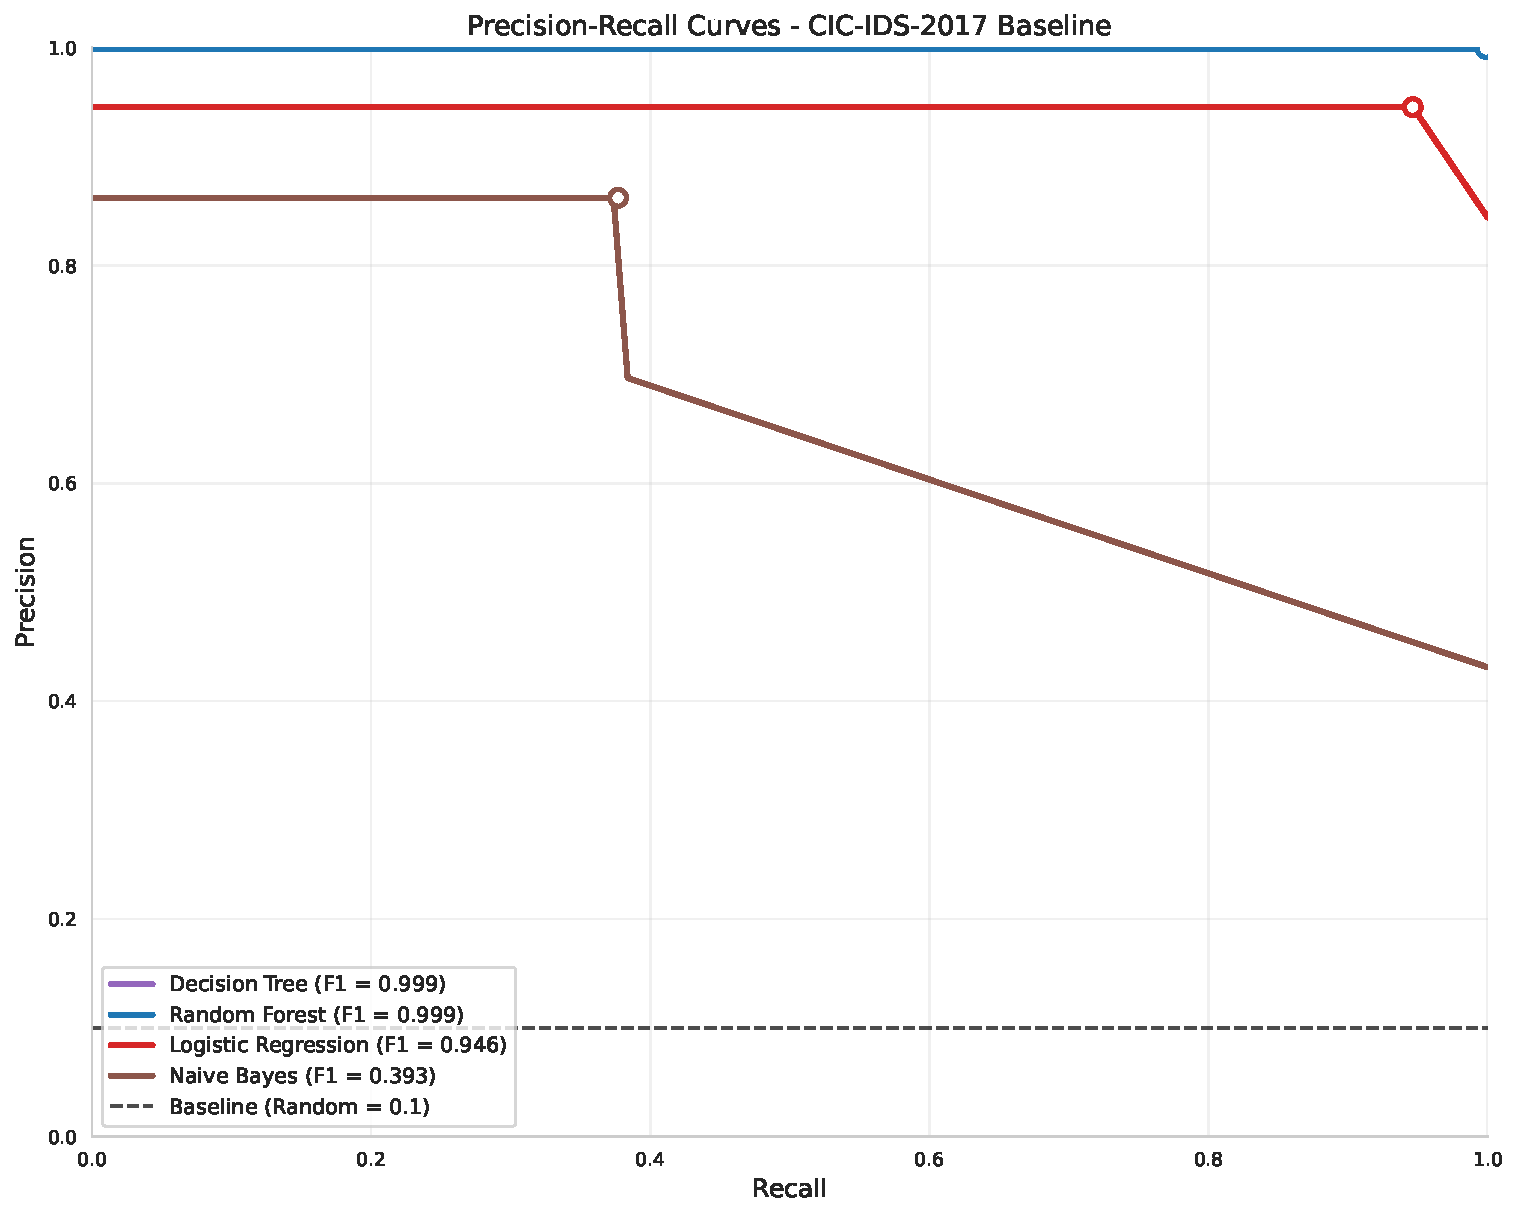
\includegraphics[width=\textwidth]{../data/results/precision_recall_curves/cic_ids_2017_baseline_scientific_pr.pdf}
            \caption{CIC-IDS-2017 Baseline}
        \end{subfigure}
        \\[1em]
        \begin{subfigure}[b]{0.48\textwidth}
            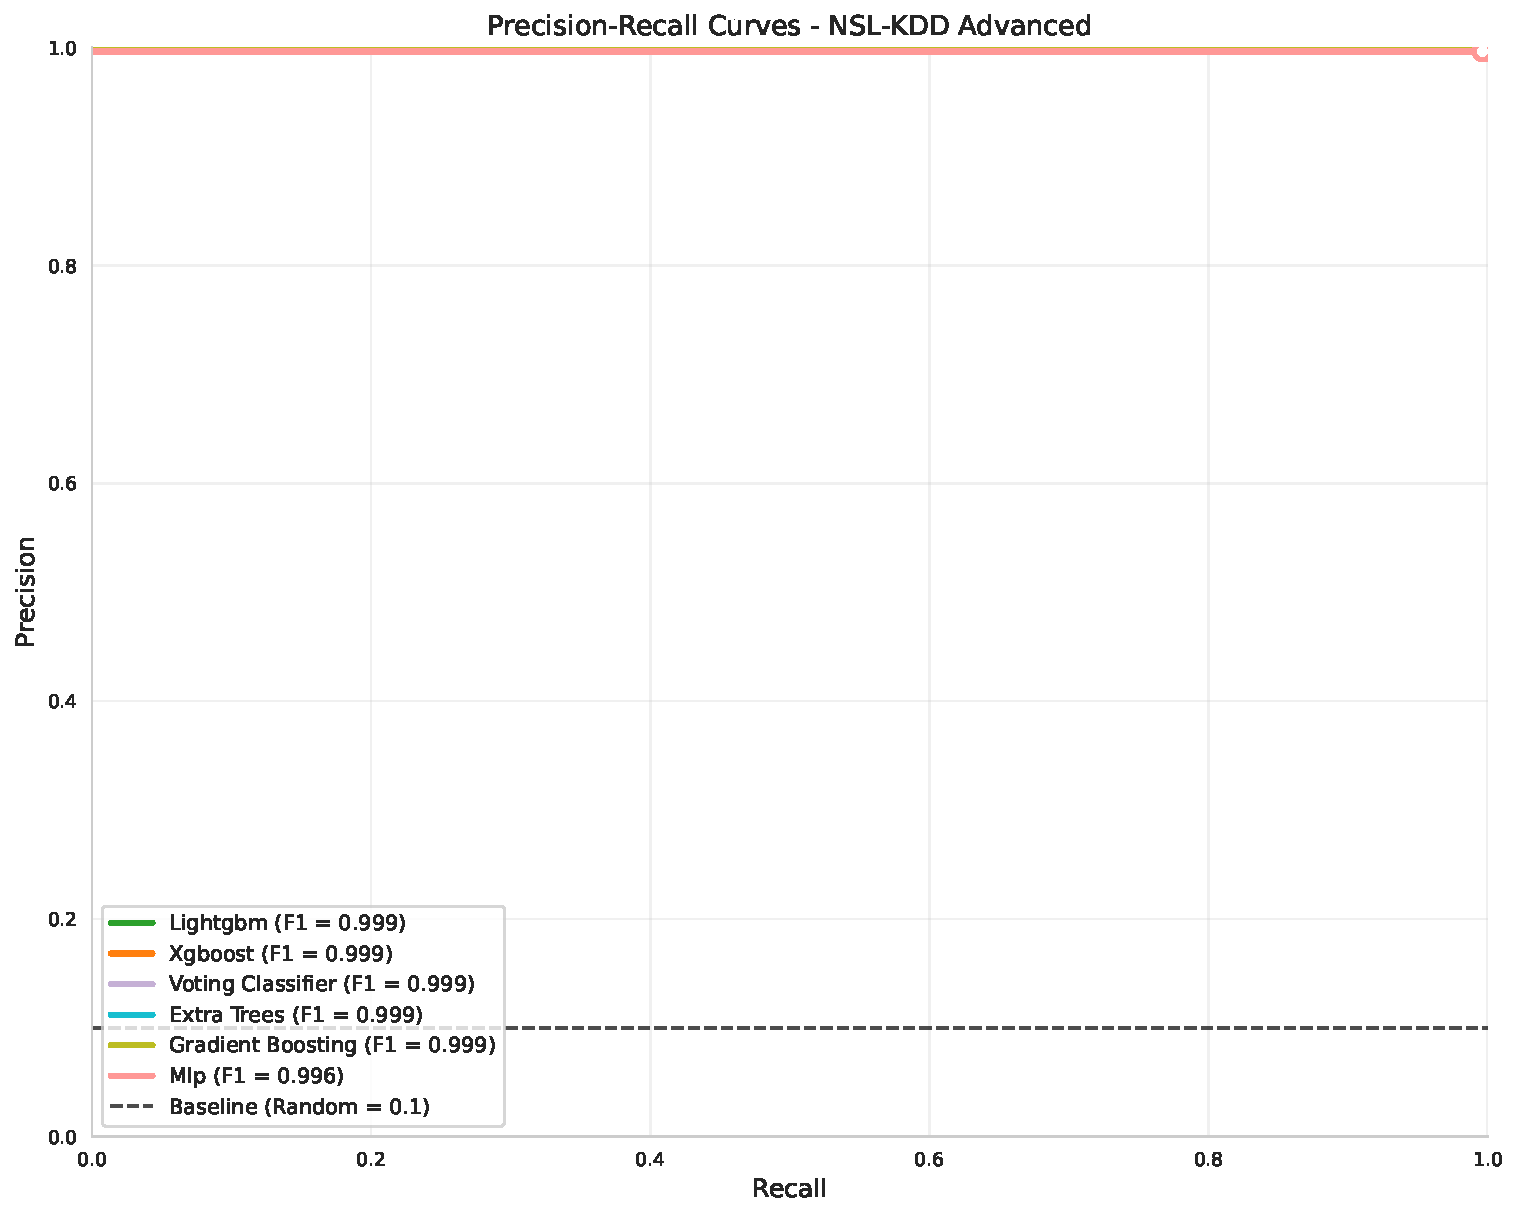
\includegraphics[width=\textwidth]{../data/results/precision_recall_curves/nsl_kdd_advanced_scientific_pr.pdf}
            \caption{NSL-KDD Advanced}
        \end{subfigure}
        \hfill
        \begin{subfigure}[b]{0.48\textwidth}
            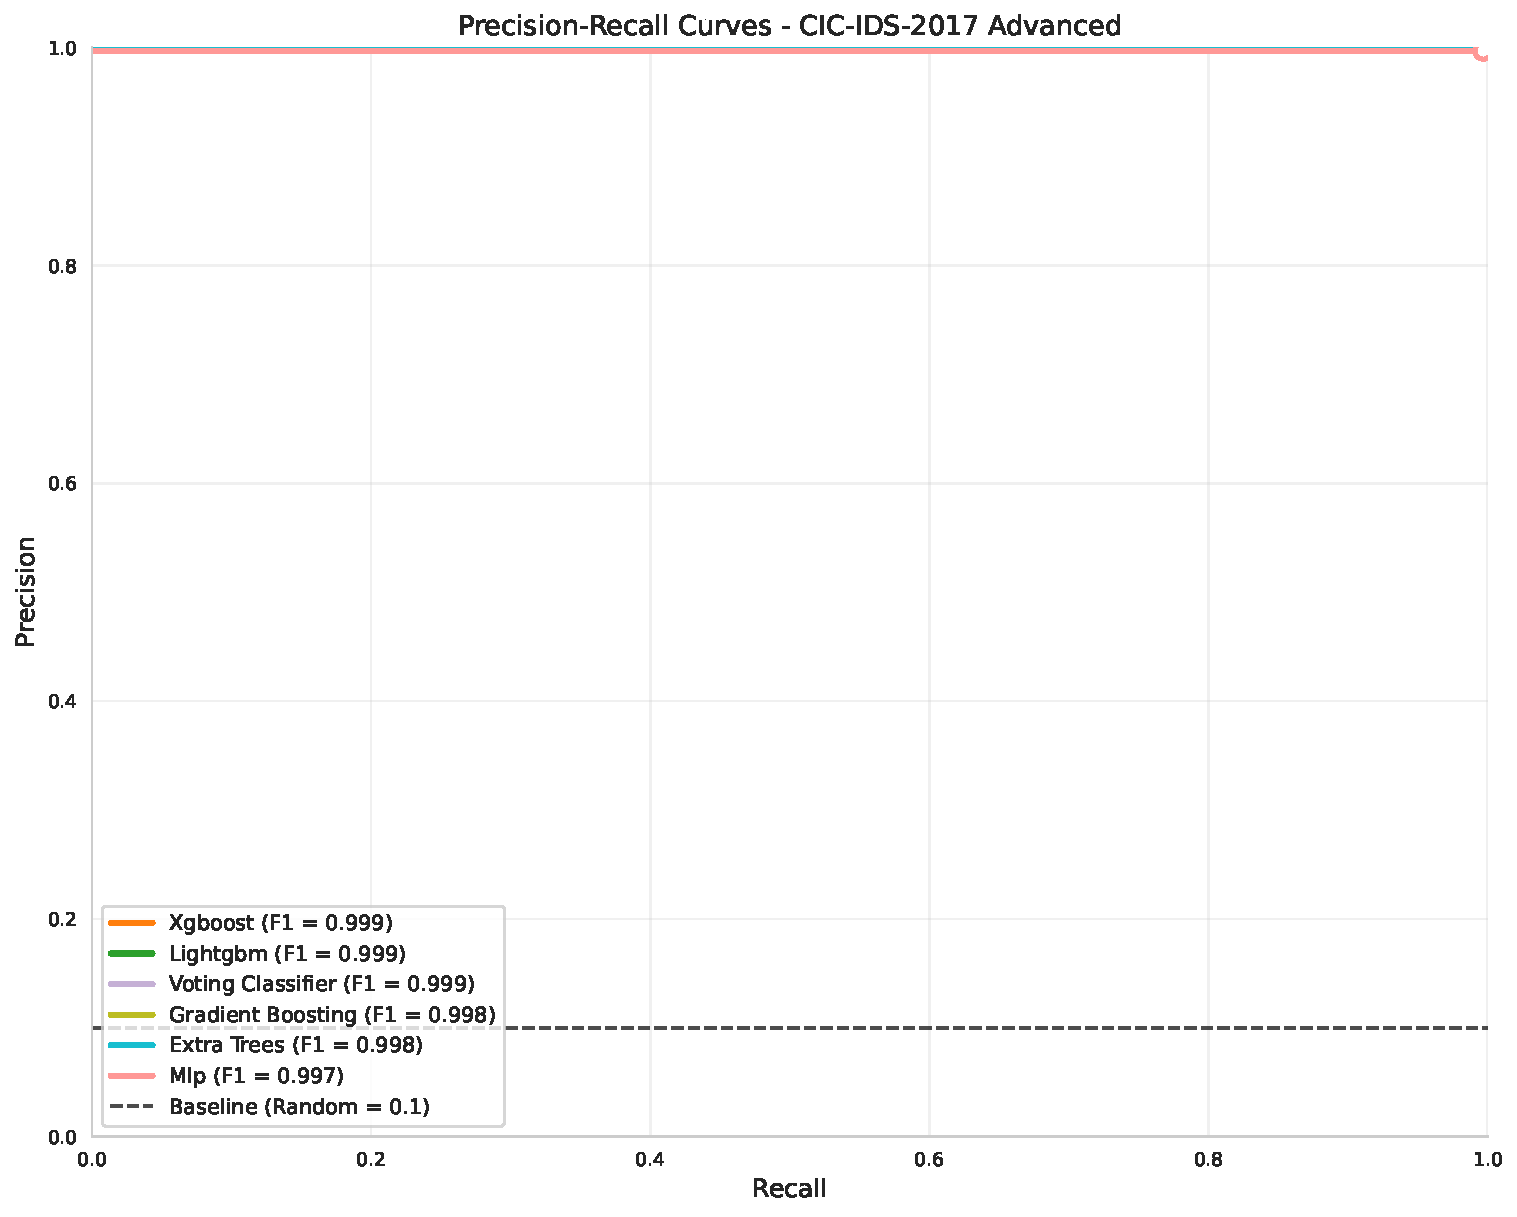
\includegraphics[width=\textwidth]{../data/results/precision_recall_curves/cic_ids_2017_advanced_scientific_pr.pdf}
            \caption{CIC-IDS-2017 Advanced}
        \end{subfigure}
        \caption{Precision-Recall Trade-Off-Analyse: PR-Kurven sind besonders 
        informativ bei Klassenimbalance (CIC: 83\% Normal). Average Precision (AP) 
        aggregiert Performance über alle Schwellenwerte. Baseline-Modelle zeigen 
        stärkeren Precision-Drop bei hohem Recall (rechte Kurvenabschnitte) im 
        Vergleich zu Advanced-Modellen.}
        \source{Eigene Darstellung.}
        \label{fig:app_pr_curves}
    \end{figure}
    
    \paragraph{PR-Kurven vs. ROC-Kurven}
    Bei starker Klassenimbalance (CIC-IDS-2017):
    \begin{itemize}
        \item \textbf{ROC-Kurven:} Können übermäßig optimistisch wirken 
        (hohe TN-Zahlen dominieren)
        \item \textbf{PR-Kurven:} Fokussieren auf Minority Class (Attack), 
        daher realistischere Einschätzung
        \item \textbf{Beispiel:} Random Forest CIC-IDS hat ROC-AUC = 1.0, 
        aber AP = 0.999 (minimale Precision-Degradation bei hohem Recall)
    \end{itemize}
    
    \subsection{Konfusionsmatrizen NSL-KDD}
    \label{app:cm_nsl}
    
    \begin{figure}[H]
        \centering
        \begin{subfigure}[b]{0.48\textwidth}
            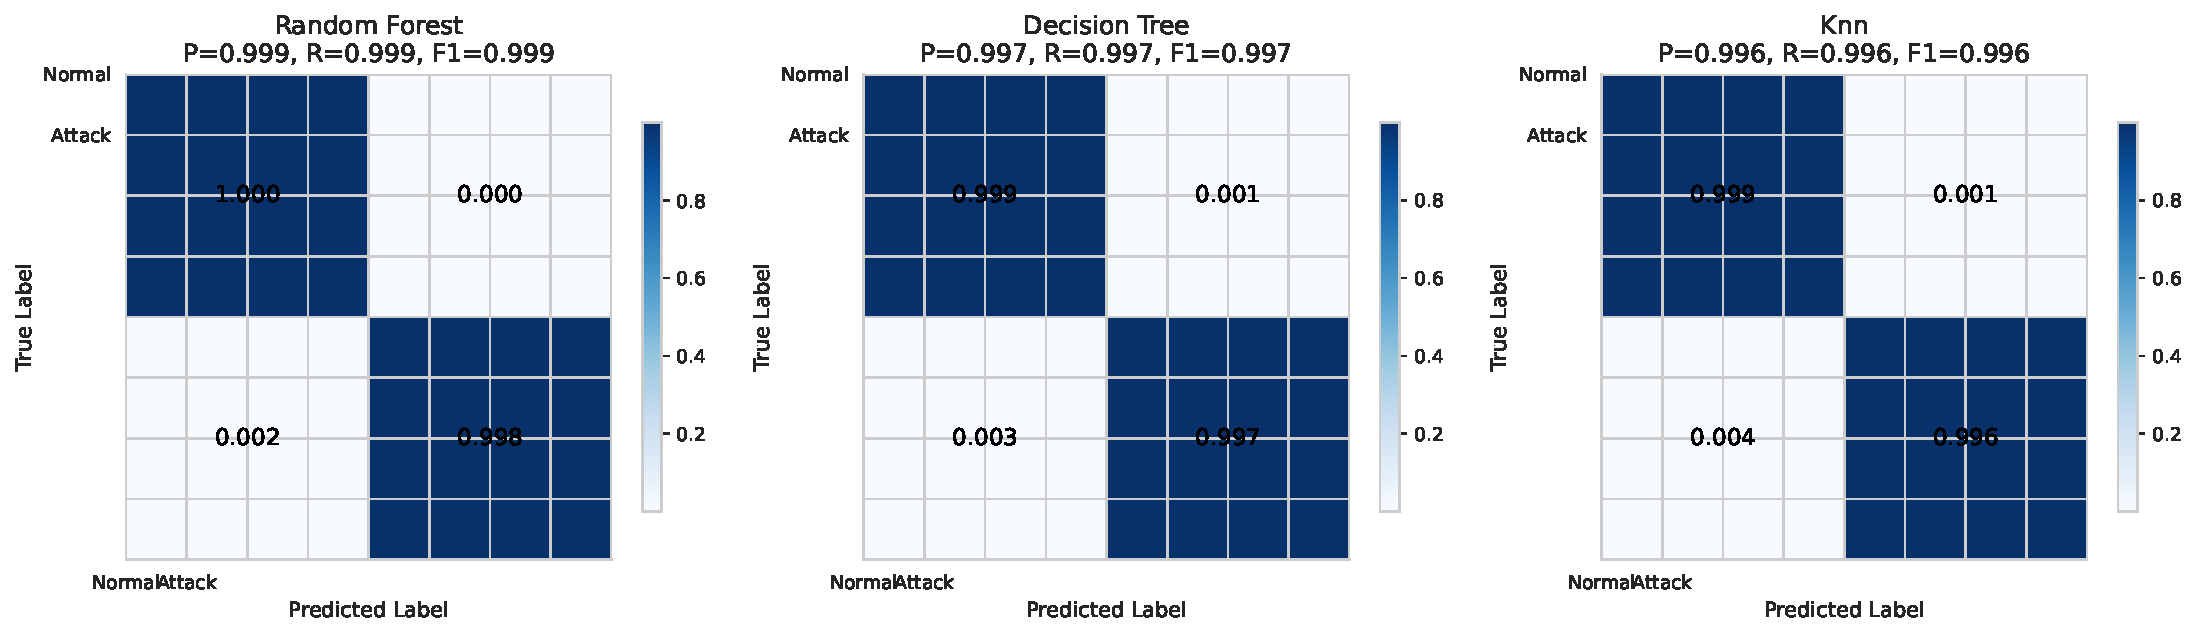
\includegraphics[width=\textwidth]{../data/results/confusion_matrices/nsl_kdd_baseline_scientific_cm.pdf}
            \caption{Baseline-Modelle}
        \end{subfigure}
        \hfill
        \begin{subfigure}[b]{0.48\textwidth}
            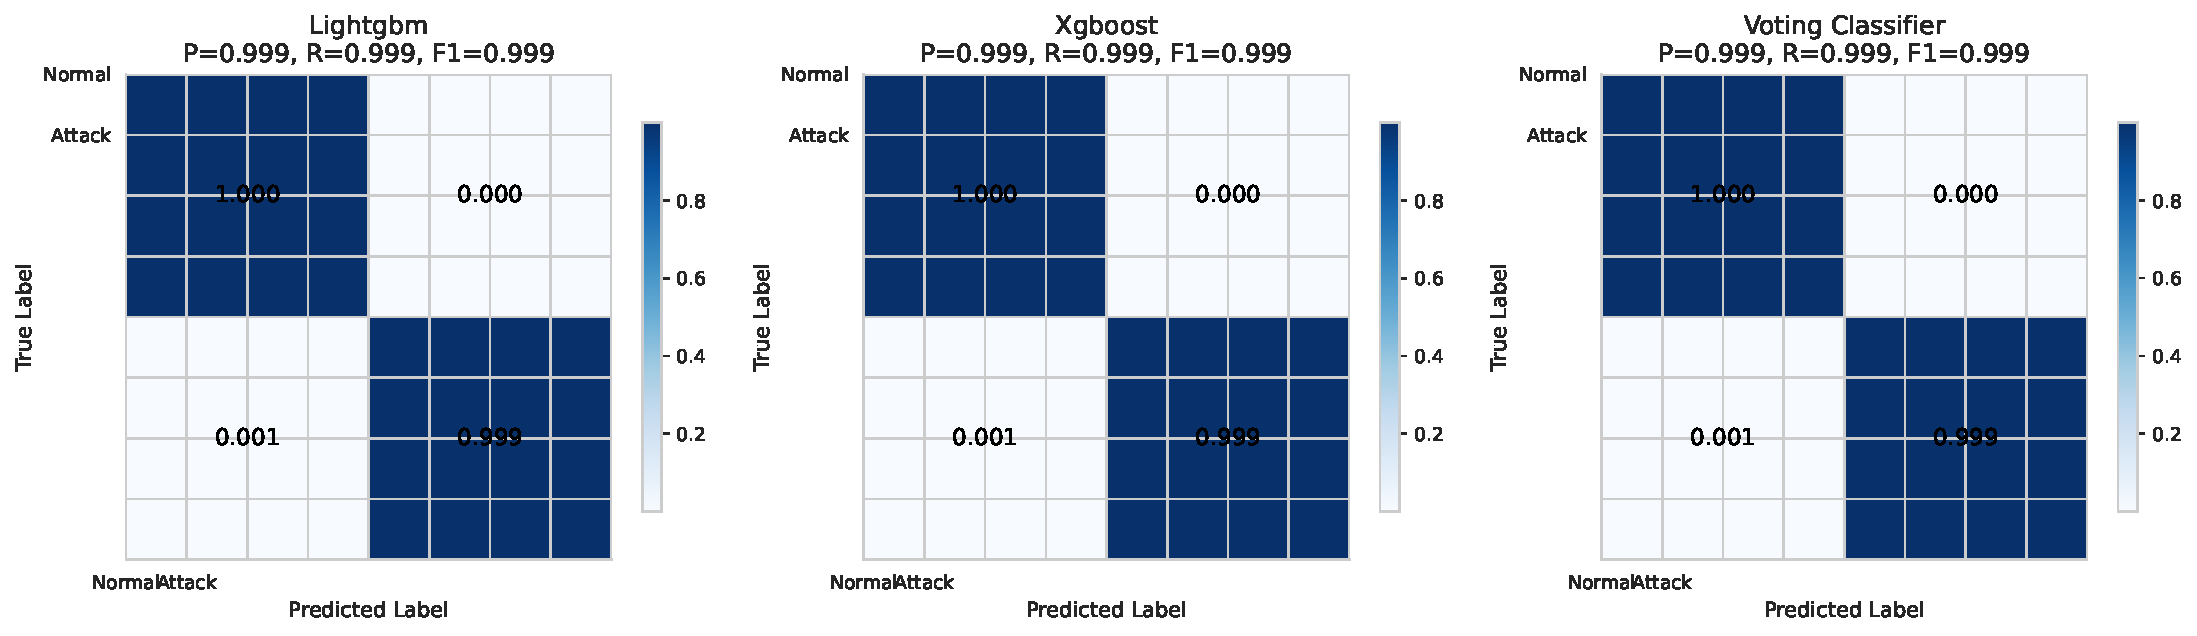
\includegraphics[width=\textwidth]{../data/results/confusion_matrices/nsl_kdd_advanced_scientific_cm.pdf}
            \caption{Advanced-Modelle}
        \end{subfigure}
        \caption{Konfusionsmatrizen NSL-KDD (normalisiert pro True Label): 
        Diagonalelemente = korrekte Klassifikationen (idealer Wert: 1.0). 
        SVM-Linear zeigt starke False-Negative-Rate (dunklere Off-Diagonal-Werte).}
        \source{Eigene Darstellung.}
        \label{fig:app_cm_nsl}
    \end{figure}
    
    \subsection{Konfusionsmatrizen CIC-IDS-2017}
    \label{app:cm_cic}
    
    \begin{figure}[H]
        \centering
        \begin{subfigure}[b]{0.48\textwidth}
            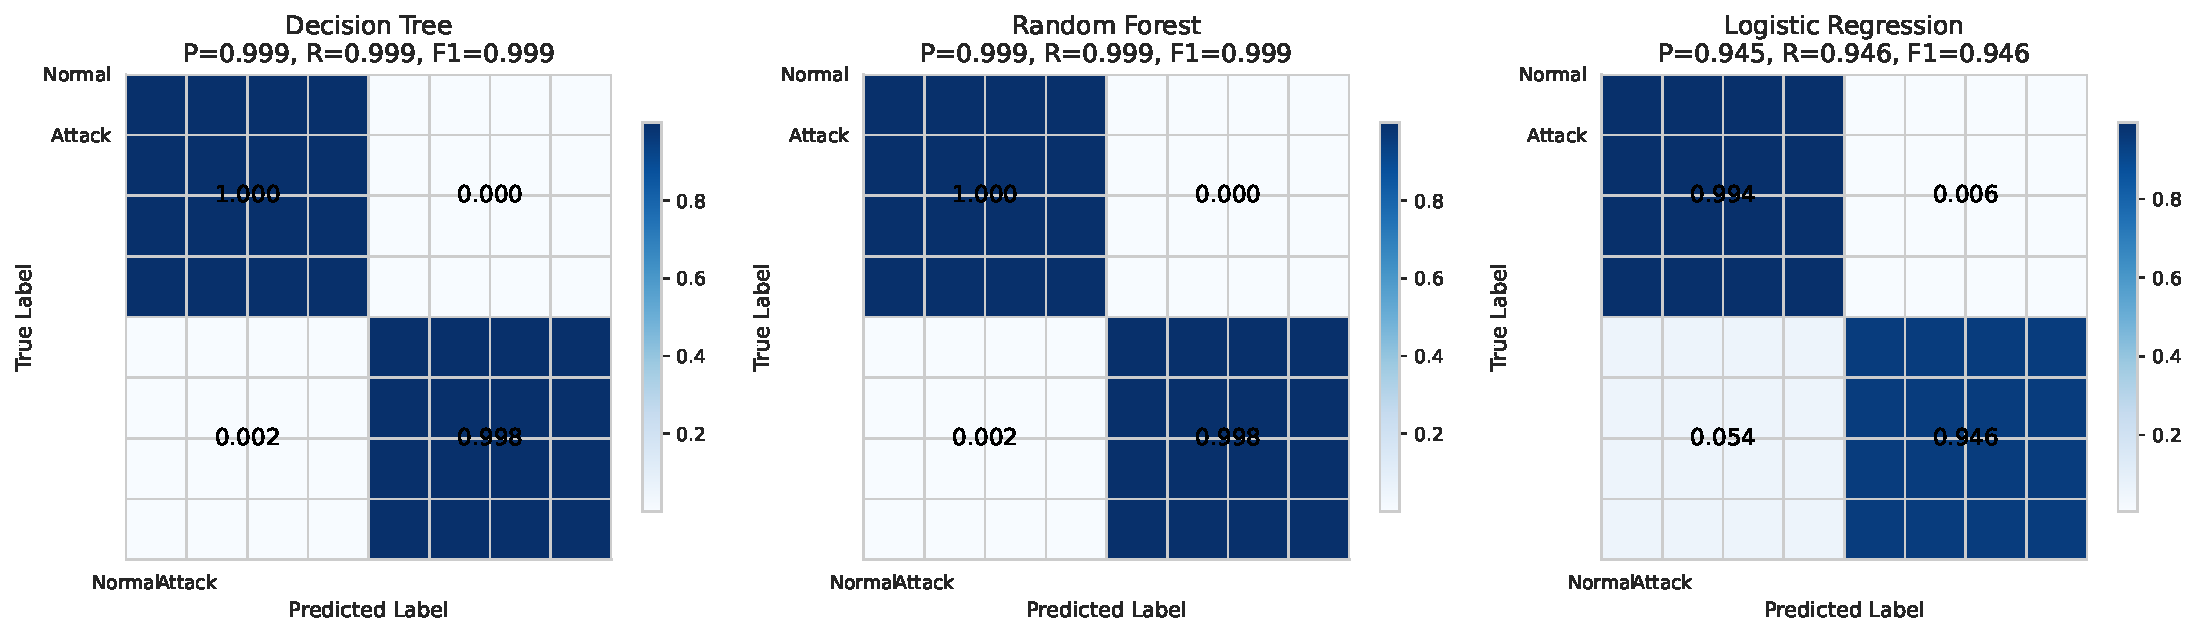
\includegraphics[width=\textwidth]{../data/results/confusion_matrices/cic_ids_2017_baseline_scientific_cm.pdf}
            \caption{Baseline-Modelle}
        \end{subfigure}
        \hfill
        \begin{subfigure}[b]{0.48\textwidth}
            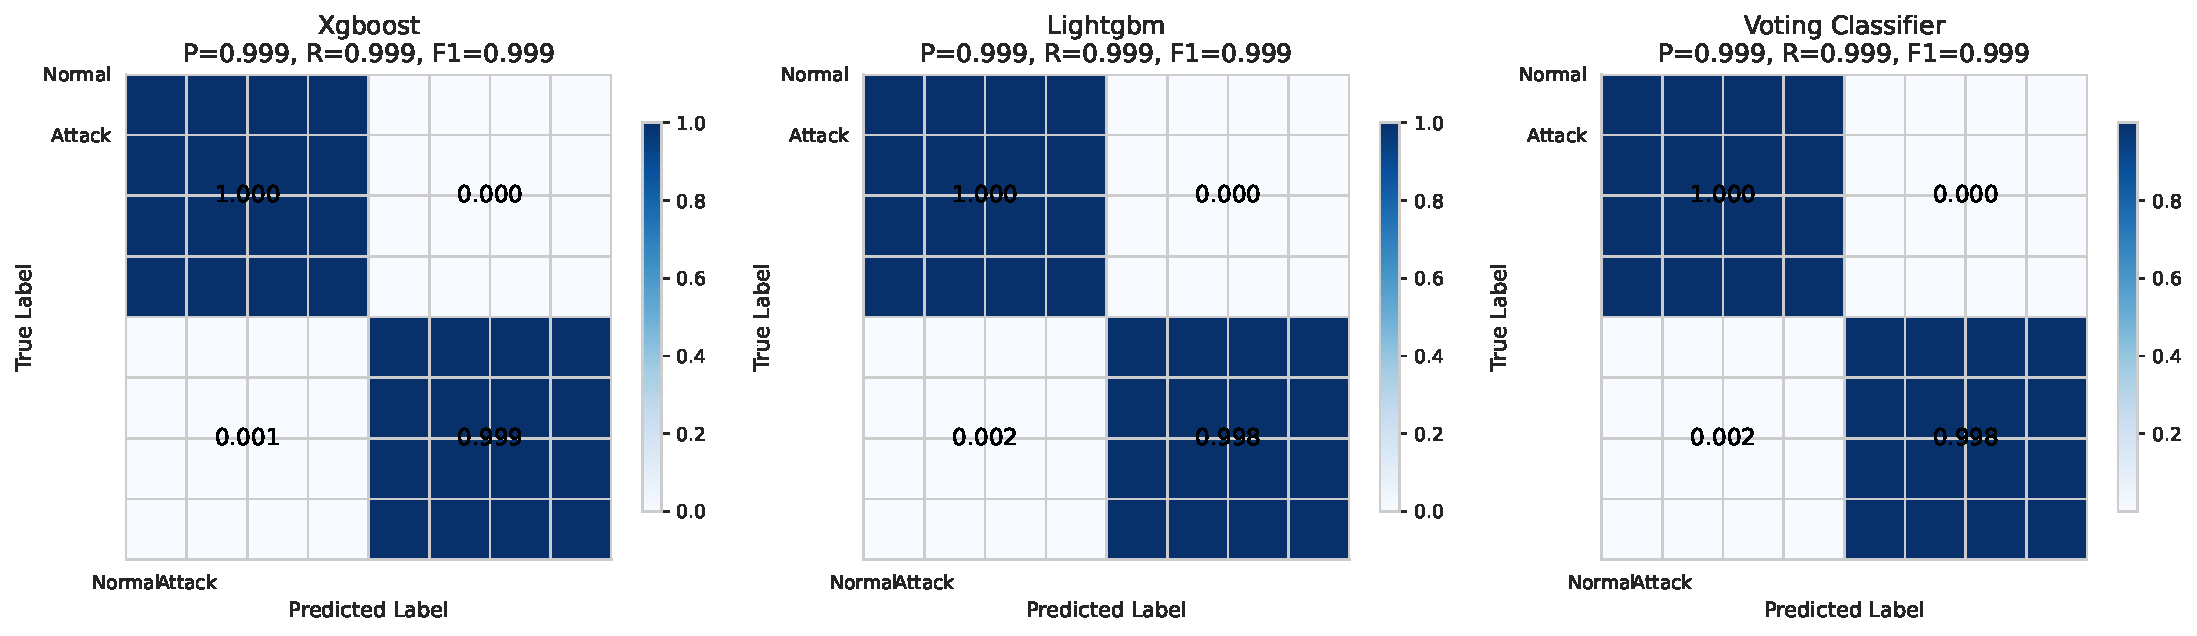
\includegraphics[width=\textwidth]{../data/results/confusion_matrices/cic_ids_2017_advanced_scientific_cm.pdf}
            \caption{Advanced-Modelle}
        \end{subfigure}
        \caption{Konfusionsmatrizen CIC-IDS-2017: Naive Bayes zeigt charakteristische 
        Bias zur Attack-Klasse (hohe False-Positive-Rate bei Normal $\rightarrow$ 
        Attack), während Decision Tree nahezu perfekte Klassifikation erreicht 
        (Diagonale $\approx$ 1.0).}
        \source{Eigene Darstellung.}
        \label{fig:app_cm_cic}
    \end{figure}
    
    \section{Pseudocode}
    (Optionaler Inhalt des Anhangs.)

        % ---------- Nützliche LaTeX-Referenz ----------

    \clearpage
    \section*{Nützliche LaTeX-Referenz}
    \addtoTOC{Nützliche LaTeX-Referenz}

    \subsection*{Zitieren nach APA 7 (biblatex-apa)}
    Indirektes Zitat: \verb|\parencite{Goodfellow2016}| → (Goodfellow et al., 2016)\\
    Mit Seitenzahl: \verb|\parencite[S.~123]{Bishop2006}|\\
    Direktzitat ≤40 Wörter: „…“ \verb|\parencite[S.~45]{Hastie2009}|\\
    Blockzitat ≥40 Wörter:

    \begin{verbatim}
        \begin{blockzitat}
            Langes Zitat ohne Anführungszeichen …
        \end{blockzitat}
    \end{verbatim}

    \subsection*{Abbildungen}
    \begin{verbatim}
        \begin{figure}[h]
            \centering
            \includegraphics[width=0.85\textwidth]{pfad/zur/datei}
            \caption{Titel der Abbildung.}
            \source{Quelle: Eigene Darstellung / Autor, Jahr, S.~xx.}
            \label{fig:beispiel}
        \end{figure}
    \end{verbatim}
    Querverweis: „siehe Abb.~\verb|\ref{fig:beispiel}|“.

    \subsection*{Tabellen}
    \begin{verbatim}
        \begin{table}[h]
            \centering
            \begin{tabular}{lcc}
                \toprule
                \textbf{Variable} & \textbf{Gruppe A} & \textbf{Gruppe B} \\
                \midrule
                x & 1{,}23 & 4{,}56 \\
                \bottomrule
            \end{tabular}
            \caption{Titel der Tabelle.}
            \source{Quelle: Eigene Darstellung.}
            \label{tab:beispiel}
        \end{table}
    \end{verbatim}
    Querverweis: „siehe Tab.~\verb|\ref{tab:beispiel}|“.

    \subsection*{Gleichungen}
    Einzeln:
    \begin{verbatim}
        \begin{equation}
            E = mc^2
        \end{equation}
    \end{verbatim}

    Mehrzeilig (nummeriert):
    \begin{verbatim}
        \begin{align}
            \hat{R}(\theta) &= \frac{1}{N}\sum_{i=1}^{N}\ell(y_i,f_\theta(x_i)) + \lambda\lVert\theta\rVert_2^2,\\
            \ell(y,\hat{y}) &= -\big[y\log\hat{y} + (1-y)\log(1-\hat{y})\big].
        \end{align}
    \end{verbatim}

    \subsection*{Listen}
    \begin{verbatim}
        \begin{itemize}
            \item Punkt A
            \item Punkt B
        \end{itemize}

        \begin{enumerate}
            \item Erstens
            \item Zweitens
        \end{enumerate}
    \end{verbatim}

    \subsection*{Fußnoten}
    \verb|Text\footnote{Inhalt der Fußnote in 10 pt.}|

    \subsection*{Einheiten und Zahlen (siunitx)}
    \verb|\SI{12,5}{\kilo\meter\per\hour}| → \SI{12,5}{\kilo\meter\per\hour}\\
    \verb|\num{12345,678}| → \num{12345,678}

    \subsection*{Quellen in Abbildungen/Tabellen}
    Direkt unter \verb|\caption| einfügen: \verb|\source{Quelle: …}| (10 pt).

    \subsection*{Platzhalter \& Blindtext}
    Platzhalterbild: \verb|\includegraphics{example-image}| (aus Paket \verb|mwe|).\\
    Kurzer Blindtext:
    \begin{verbatim}
        Lorem ipsum dolor sit amet, consectetur adipiscing elit.
    \end{verbatim}

    \subsection*{Bibliografie-Einträge (BibTeX mit Biber)}
    \textbf{Wichtige Eintragstypen:}
    \begin{verbatim}
@book{key,
  author = {Nachname, Vorname},
  year = {2023},
  title = {Titel des Buches},
  subtitle = {Untertitel (optional)},
  publisher = {Verlag},
  address = {Ort},
  edition = {2}, % nur bei 2. Auflage oder höher
  doi = {10.1000/xyz}
}

@article{key,
  author = {Nachname, Vorname and Zweiter, Autor},
  year = {2023},
  title = {Titel des Artikels},
  journaltitle = {Name der Zeitschrift},
  volume = {42},
  number = {3},
  pages = {123--145},
  doi = {10.1000/xyz}
}

@online{key,
  author = {Nachname, Vorname},
  year = {2023},
  title = {Titel der Webseite},
  url = {https://example.com},
  urldate = {2024-01-15}
}
    \end{verbatim}

    \textbf{Biber-spezifische Felder:}
    \begin{itemize}
        \item \verb|journaltitle| statt \verb|journal| (APA-konform)
        \item \verb|location| statt \verb|address| (moderne biblatex-Syntax)
        \item \verb|date| statt \verb|year| für komplexere Datumsangaben
    \end{itemize}

\subsection*{Code-Beispiele in LaTeX}

\textbf{Einfacher Python-Code:}

\begin{lstlisting}[language=Python, caption={Fibonacci-Beispiel}, label={lst:fib}]
    def fibonacci(n: int) -> list[int]:
    """Berechnet die ersten n Fibonacci-Zahlen."""
    seq = [0, 1]
    for i in range(2, n):
    seq.append(seq[-1] + seq[-2])
    return seq[:n]


    if __name__ == "__main__":
    print("Fibonacci(10):", fibonacci(10))
\end{lstlisting}

\textbf{Ausgabe:}
\begin{verbatim}
    Fibonacci(10): [0, 1, 1, 2, 3, 5, 8, 13, 21, 34]
\end{verbatim}

---

\textbf{Inline-Nutzung (LaTeX-Syntax wörtlich):}
\begin{verbatim}
    \begin{lstlisting}[language=Python, caption={Minimalbeispiel}, label={lst:mini}]
        def foo(x):
        return x**2
    \end{lstlisting}
\end{verbatim}

\textbf{Tatsächliches Listing (ausführbarer Code):}
\begin{lstlisting}[caption={Minimalbeispiel}, label={lst:mini}]
    def foo(x):
    return x**2
\end{lstlisting}

\textbf{Ausgabe:}
\begin{verbatim}
    >>> foo(5)
    25
\end{verbatim}

    ---

    \textbf{Code aus Datei einbinden:}
    \lstinline[language=TeX]|\lstinputlisting[language=Python, caption={Script X}, label={lst:scriptx}]{path/to/script.py}|




    \subsection*{Erweiterte LaTeX-Tipps}

    \textbf{Mathematik:}
    \begin{itemize}
        \item Inline-Mathe: \verb|$E = mc^2$| → $E = mc^2$
        \item Display-Mathe: \verb|\[E = mc^2\]| (unnummeriert)
        \item Nummerierte Gleichung: \verb|\begin{equation}...\end{equation}|
        \item Griechische Buchstaben: \verb|\alpha, \beta, \gamma| → $\alpha, \beta, \gamma$
    \end{itemize}

    \textbf{Querverweise:}
    \begin{itemize}
        \item Label setzen: \verb|\label{fig:beispiel}|
        \item Verweis: \verb|\ref{fig:beispiel}| oder \verb|\autoref{fig:beispiel}|
        \item Seitenverweis: \verb|\pageref{fig:beispiel}|
    \end{itemize}

    \textbf{Typografie:}
    \begin{itemize}
        \item Geschützte Leerzeichen: \verb|Abb.~\ref{fig:1}|
        \item Anführungszeichen: \verb|\enquote{Text}| (sprachabhängig)
        \item Gedankenstrich: \verb|--| (Bindestrich), \verb|---| (Gedankenstrich)
        \item Auslassungspunkte: \verb|\ldots| → …
    \end{itemize}

    \textbf{Häufige Probleme und Lösungen:}
    \begin{itemize}
        \item Biber-Cache löschen: \verb|biber --cache-clear|
        \item Umlaute: Verwende \verb|fontspec| mit LuaLaTeX/XeLaTeX
        \item Lange URLs: \verb|\url{...}| oder \verb|\href{url}{Text}|
        \item Overfull hbox: \verb|\sloppy| oder manuelle Zeilenumbrüche
    \end{itemize}

    \subsection*{Kompilierreihenfolge mit Biber}
    \textbf{Standard:} LuaLaTeX → Biber → LuaLaTeX → LuaLaTeX

    \textbf{VS Code/Automatisierung:}
    \begin{itemize}
        \item LaTeX Workshop Extension konfigurieren
        \item \verb|latexmkrc| für automatische Biber-Ausführung
        \item Overleaf nutzt automatisch die richtige Reihenfolge
    \end{itemize}


    % ========= Ende =========
\end{document}
